% !TeX program = pdflatex
\documentclass[a4paper,12pt]{report}

% Pakete
\usepackage[utf8]{inputenc}
\usepackage[T1]{fontenc}
\usepackage{amsmath, amssymb, amsfonts}
\usepackage[ngerman]{babel}
\usepackage{geometry}
\usepackage{graphicx}  % draft: zeigt fehlende Bilder als Rahmen
\usepackage{hyperref}
\usepackage{listings}
\usepackage{color}
\usepackage{booktabs}
\usepackage{setspace}
\usepackage{parskip}
\usepackage{acronym}
\usepackage{caption}
\usepackage{float}
\usepackage[backend=biber, style=numeric, sorting=none]{biblatex}
\addbibresource{Literatur.bib}  % Deine .bib-Datei
\geometry{left=2.5cm, right=2.5cm, top=2.5cm, bottom=2.5cm}
\graphicspath{{abbildungen/}}
\setstretch{1.25}

% Farben für Code-Listings
\definecolor{codegreen}{rgb}{0,0.6,0}
\definecolor{codegray}{rgb}{0.5,0.5,0.5}
\definecolor{codepurple}{rgb}{0.58,0,0.82}
\definecolor{backcolour}{rgb}{0.95,0.95,0.92}

\lstdefinestyle{mystyle}{
    backgroundcolor=\color{backcolour},
    commentstyle=\color{codegreen},
    keywordstyle=\color{magenta},
    numberstyle=\tiny\color{codegray},
    stringstyle=\color{codepurple},
    basicstyle=\ttfamily\footnotesize,
    breakatwhitespace=false,
    breaklines=true,
    captionpos=b,
    keepspaces=true,
    numbers=left,
    numbersep=5pt,
    showspaces=false,
    showstringspaces=false,
    showtabs=false,
    tabsize=2
}
\lstset{style=mystyle}

% Metadaten
\title{Einsatz von Large Language Models im Umfeld der Robotik hinsichtlich On-Premise-Lösungen}
\author{Moritz Jahn \\ Matrikelnummer: 3221169}
\date{\today}

\begin{document}

% ============================================================
% Titelseite und Verzeichnisse
% ============================================================
\pagenumbering{roman}
\maketitle

\tableofcontents
\cleardoublepage

\listoffigures
\cleardoublepage

\listoftables
\cleardoublepage

% ============================================================
% Abkürzungsverzeichnis
% ============================================================
\chapter*{Abkürzungsverzeichnis}
\addcontentsline{toc}{chapter}{Abkürzungsverzeichnis}
\begin{acronym}[VRAM]
    \acro{LLM}{Large Language Model}
    \acro{VLM}{Visual Language Model}
    \acro{NLP}{Natural Language Processing}
    \acro{GPU}{Graphics Processing Unit}
    \acro{CPU}{Central Processing Unit}
    \acro{VRAM}{Video Random Access Memory}
    \acro{RAM}{Random Access Memory}
    \acro{ROS}{Robot Operating System}
    \acro{API}{Application Programming Interface}
    \acro{TTS}{Text-to-Speech}
    \acro{STT}{Speech-to-Text}
    \acro{RAG}{Retrieval-Augmented Generation}
    \acro{GGUF}{GPT-Generated Unified Format}
\end{acronym}

\cleardoublepage
\pagenumbering{arabic}

% ============================================================
% Kapitelimporte
% ============================================================
% ============================================================
% Kapitel 1: Einführung
% ============================================================
\chapter{Einführung}

Kaum ein anderes Thema hat die Technologiebranche in den letzten Jahren so geprägt wie künstliche Intelligenz.
Um im globalen Wettbewerb um die leistungsfähigsten Sprachmodelle bestehen zu können, investieren
Unternehmen Milliardensummen in Recheninfrastruktur.
Ein eindrückliches Beispiel hierfür ist \textit{Colossus}, der von Elon Musks KI-Firma xAI errichtete GPU-Cluster:
Mit 100\,000 NVIDIA HGX H100 GPUs, verteilt auf vier wassergekühlte Hallen in Memphis, Tennessee, stellt er den bislang größten KI-Supercomputer der Welt dar und dient dem Training des generativen Modells Grok~\cite{brendel2025colossus}.
Die für solche Systeme benötigte Hardware stammt nahezu ausschließlich vom Branchenführer NVIDIA, der über 90\,\% des Marktes für KI-GPUs hält.
CEO Jensen Huang bezifferte das Auftragsvolumen des Unternehmens für die Jahre 2025 und 2026 auf rund 500 Milliarden US-Dollar -- ein Zeichen für die nach wie vor rasant wachsende Nachfrage~\cite{leswing2025nvidia}.
Dieser massive Ausbau von Rechenzentren hat weitreichende energetische Konsequenzen:
Laut einer Prognose der Internationalen Energieagentur (IEA) könnte sich der weltweite Stromverbrauch von Rechenzentren bis 2030 verdoppeln, wobei der Bedarf sogenannter beschleunigter Server -- wie sie für KI-Workloads eingesetzt werden -- im Zeitraum 2025 bis 2030 um 225\,\% steigt~\cite{janson2025rechenzentren}.

Angesichts dieser Entwicklungen stellt sich die Frage, ob der Betrieb solcher ressourcenintensiver Modelle für jeden Anwendungsfall notwendig ist.
Insbesondere in industriellen Einsatzszenarien -- etwa auf Edge-Geräten oder Robotern in der Produktion, die häufig keine dauerhafte Internetverbindung wünschen oder zulassen -- bieten sich deutlich kleinere, spezialisierte Modelle an.
Diese können \textit{On-Premise}, also vor Ort auf eigener Hardware, betrieben werden und erfordern weder die enormen Rechenkapazitäten cloudbasierter Infrastrukturen noch den damit verbundenen Energieverbrauch.
Die vorliegende Arbeit untersucht daher, inwieweit solche lokalen Modelle für spezifische Anwendungsfälle eine praktikable und effiziente Alternative zu den großen, cloudbasierten Sprachmodellen darstellen.



\section{Problemstellung}

Der rasante Ausbau cloudbasierter KI-Dienste wirft neben technischen und energetischen Fragen zunehmend auch Bedenken hinsichtlich \textbf{Datenhoheit}, \textbf{Sicherheit} und \textbf{technologischer Unabhängigkeit} auf.
Die dominierenden KI-Plattformen -- darunter Dienste von OpenAI, Google und Anthropic -- werden überwiegend in Rechenzentren US-amerikanischer Hyperscaler betrieben.
Daten, die an diese Modelle übermittelt werden, verlassen damit häufig den europäischen Rechtsraum und unterliegen potenziell dem Zugriff ausländischer Behörden, etwa im Rahmen des US-amerikanischen CLOUD Act.
Laut dem Bitkom Cloud Report 2025 sehen 78\,\% der deutschen Unternehmen eine zu starke Abhängigkeit von US-Cloud-Anbietern, und für 97\,\% der befragten Cloud-Nutzer spielt die Herkunft des Anbieters bei der Auswahl eine wesentliche Rolle~\cite{bitkom2025cloud}.

Für produzierende Unternehmen verschärft sich diese Problematik zusätzlich:
Sensible Produktionsdaten, Prozessparameter oder Qualitätsinformationen dürfen aus Gründen des Geschäftsgeheimnisschutzes und der Compliance häufig das Unternehmensnetzwerk nicht verlassen.
Roboter und Edge-Geräte in der Fertigung operieren zudem oft in Umgebungen ohne zuverlässige oder gewünschte Internetanbindung.
Die Nutzung cloudbasierter KI-Modelle ist in solchen Szenarien daher entweder nicht möglich oder mit erheblichen Risiken verbunden.
Es stellt sich somit die Frage, ob kleinere, spezialisierte Sprachmodelle, die vollständig vor Ort, also On-Premise, betrieben werden können, eine sichere, unabhängige und zugleich leistungsfähige Alternative für industrielle Anwendungsfälle darstellen. Bevor jedoch auf die Problematik eingegangen wird, wird im folgenden Kapitel der Stand der Technik erläutert.

\section{Stand der Technik}

Wie im vorherigen Kapitel bereits aufgegriffen, beschäftigt sich diese Arbeit primär mit der Verwendung von Large Language Models auf Edge"=Geräten und On"=Premise"=Infrastrukturen.
Der Begriff des maschinellen Lernens ist in der Informatik keineswegs neu -- bereits seit Anfang des 21.\ Jahrhunderts existieren Algorithmen, die nichtlineare Zusammenhänge in Daten erkennen können.
Einen entscheidenden Durchbruch markierte das Jahr 2017, als Vaswani et al.\ die sogenannte Transformer"=Architektur vorstellten.
Diese Architektur ermöglichte den Übergang von sequenzieller zu paralleler Datenverarbeitung und erlaubte es, diese Parallelisierung mit der massiven Rechenleistung moderner GPUs zu koppeln, um deutlich größere Datenmengen effizient zu verarbeiten.

Auf dieser Grundlage entstanden Modelle, die in der Lage sind, komplexe Muster in umfangreichen Textkorpora zu erkennen und natürlichsprachliche Ausgaben zu erzeugen -- sogenannte \textit{Large Language Models} (LLMs).
Laut Kasneci et al.\ (2023) ist ein LLM ein künstliches Intelligenzsystem, das auf einer riesigen Menge von Textdaten trainiert wurde, um natürliche Sprache zu interpretieren und menschenähnliche Antworten auf textbasierte Eingabeaufforderungen oder Fragen zu generieren~\cite{llm_definition}.

Seitdem hat sich die Leistungsfähigkeit dieser Modelle rasant weiterentwickelt, wobei die Parameteranzahl und damit auch der Ressourcenbedarf stetig gestiegen sind.
In Abbildung~\ref{fig:vram_llm} werden die geschätzten Mengen an schnell zugänglichem Grafikspeicher (VRAM) dargestellt, die für den Betrieb aktueller Flagschiffmodelle erforderlich sind.
Für Edge"=Geräte, die auf eine begrenzte Speicherkapazität angewiesen sind, kommen diese Modelle daher nicht in Frage.

\begin{figure}[H]
    \centering
    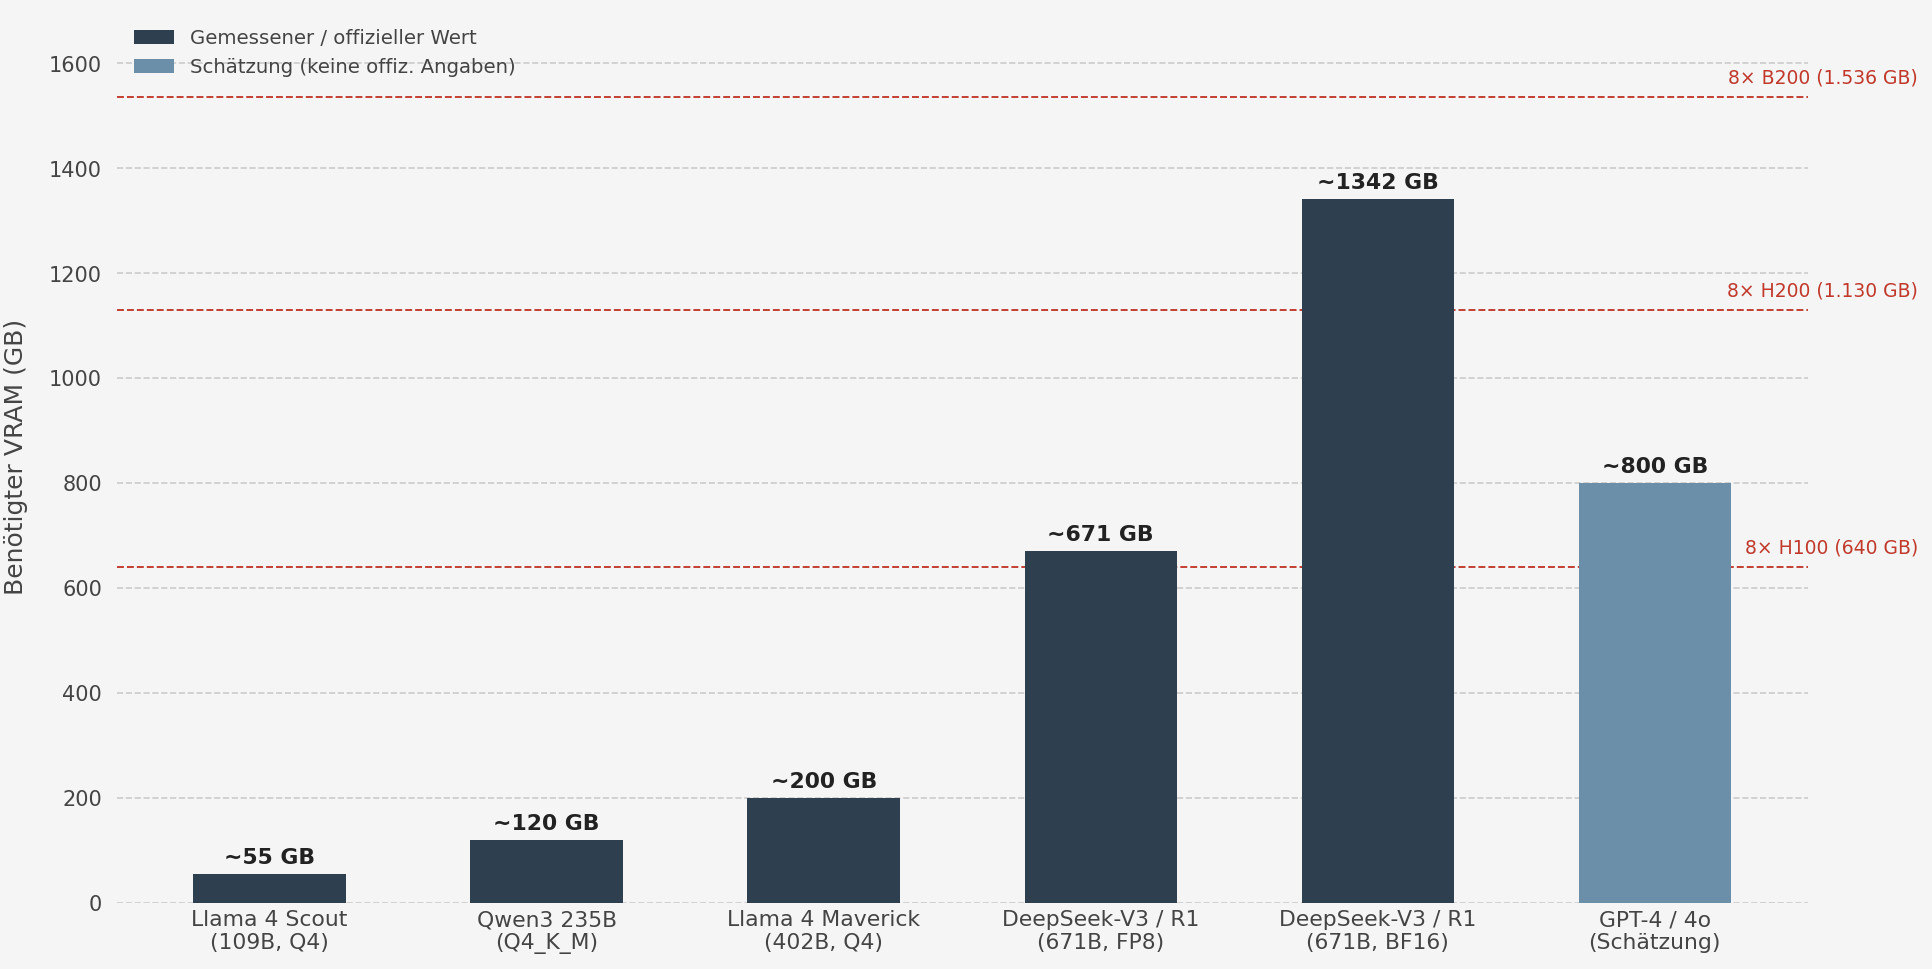
\includegraphics[width=0.83\textwidth]{abbildungen/vramllm.jpg}
    \caption{Geschätzter VRAM-Bedarf aktueller LLM-Flagschiffmodelle}
    \label{fig:vram_llm}
\end{figure}

Die leistungsstärksten quelloffenen Modelle, die für einen On"=Premise"=Betrieb relevant sind, werden in Abbildung~\ref{fig:llm_onpremise} gegenübergestellt.
Dabei wird der Chatbot-Arena-Elo-Score -- ein crowdsource-basiertes Maß für die vom Nutzer wahrgenommene Antwortqualität -- dem jeweiligen VRAM"=Bedarf bei 4"=Bit"=Quantisierung (INT4) gegenübergestellt.
Modelle, die mit maximal 48\,GB VRAM auskommen, lassen sich bereits auf einer einzelnen Consumer"=GPU betreiben und sind somit für Edge- und On"=Premise"=Szenarien besonders interessant.
Prinzipiell sind die jeweils neuesten Modellgenerationen die leistungsstärksten; zum Zeitpunkt der Erstellung dieser Arbeit stellt Qwen~3.5 von Alibaba mit einem Arena-Elo-Score von 1450 das leistungsstärkste quelloffene Modell dar.

\begin{figure}[H]
    \centering
    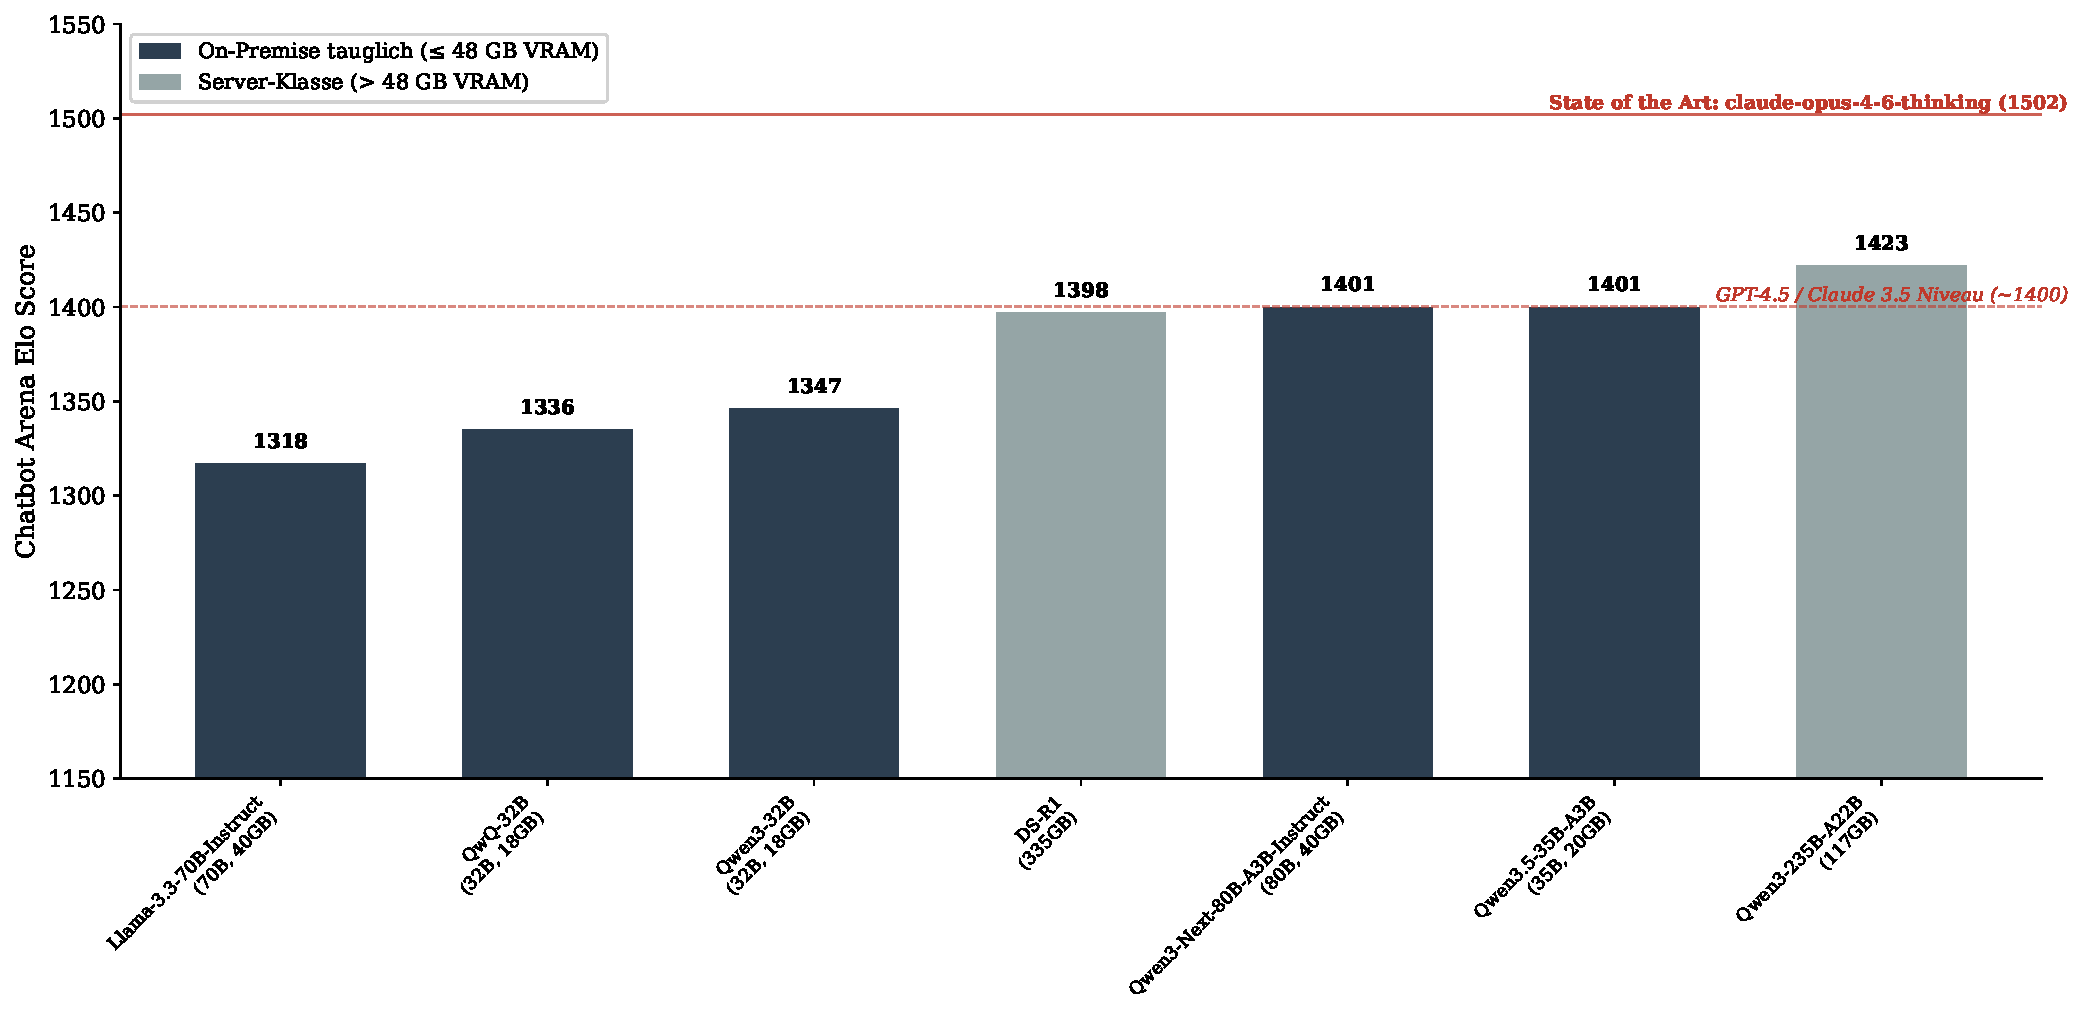
\includegraphics[width=0.95\textwidth]{abbildungen/llm_onpremise_leaderboard.pdf}
    \caption{Vergleich quelloffener LLMs: Chatbot Arena Elo vs.\ VRAM-Bedarf (INT4). Grün hervorgehobene Modelle sind für den Betrieb auf einer einzelnen Consumer-GPU ($\leq$\,48\,GB) geeignet. Datenquelle: onyx.app/self-hosted-llm-leaderboard, Stand März 2026.}
    \label{fig:llm_onpremise}
\end{figure}

\section{Zielsetzung}

Im Rahmen dieser Forschungsarbeit wird der Einsatz von On-Premise-LLMs, also vor Ort betriebenn, am Beispiel der Anwendungsmöglichkeit im Innovationszentrum für Produktion und Logistik (im folgenden IZPL) der OTH Regensburg untersucht. Dabei wird auf öffentlich verfügbare Modelle zurückgegriffen, die lokal auf einem Server des IZPL betrieben werden. Ziel ist es, die Grundlagen, technischen Anforderungen und Möglichkeiten solcher Systeme für künftige robotiknahe Anwendungen zu analysieren. Konkret dient diese wissenschaftliche Arbeit als Fundament für eine Abschlussarbeit im IZPL Regensburg.


\section{Aufbau der Arbeit}

Zunächst erfolgt eine Einführung in die mathematischen Konzepte, auf denen die Modelle basieren. Die im Folgenden aufgeführten Hardwarespezifikationen legen dar, welche Computing-Kapazitäten erforderlich sind, um sogenannte "künstliche Intelligenzen" (KI) zu erschaffen. Nach Evaluation einer Testanwendung in Kapitel 4 werden Sicherheits- und Fehlerbilder aufgezeigt. Die vorliegende Arbeit findet ihren Abschluss in Kapitel 6, das einen Ausblick auf zukünftige Forschungsgebiete gibt und ein Fazit zieht.

% ============================================================
% Kapitel 2: Grundlagen Large Language Models
% ============================================================

\chapter{Grundlagen Large Language Models}

\vspace{-0.6cm}
Dieses Kapitel legt die theoretischen Grundlagen für das Verständnis
moderner Large Language Models (LLMs). Es werden zunächst die mathematischen
Grundlagen vom Embedding bis zur Softmax-Funktion erläutert und danach eine Text to speach Pipline vorgestellt. Das Kapitel beginnt mit Abbildung \ref{fig:llm_pipeline} welche sich auf den Grundlegenden Meachanismus eines LLMs fokussiert, den Transformer. LLMs haben wie in der Überschrift ersiochtlich aus sogenannten Prompts 

\begin{figure}[H]
    \centering
    \includegraphics[width=0.43\textwidth]{LLM.png}
    \caption{Datenfluss eines Large Language Models}
    \label{fig:llm_pipeline}
\end{figure}

% ============================================================
\section{Tokenisierung und Embedding}
\label{sec:tokenisierung_embedding}
% ============================================================

Bevor jedoch der Transformer zum Einsatz kommt, ist der erste Schritt eines jeden LLMs das sogenannte Tokenisieren. Ein Token im Kontext des maschinellen Lernens wurde im Januar dieses Jahres von Daniel Jurafsky \& James H. Martin wie folgt definiert: \"`Tokens sind Einheiten, welche entstehen, nachdem wir Algorithmen wie BPE oder WordPiece anwenden, um Texteingaben für LLMs vorzubereiten."'\cite{book} In Abbildung \ref{fig:llm_pipeline} wird dieser Schritt mit dem ersten Block dargestellt und heißt übergeordnet Embedding. Beim Tokenisieren werden Wörter in Arrays umgewandelt. Zur Einordnung: Einer der ersten LLMs der Firma OpenAI, GPT-2, benutzt 768 Koordinaten, um den multidimensionalen Vektor eines einzigen Tokens aufzuspannen und um dessen Kontext zu speichern (siehe 2.1 in \cite{brown2020languagemodelsfewshotlearners}). In Abbildung \ref{fig:embedding} ist das Vektor-Embedding für den Satz \"`LLMs with Igus Rebel 6 DOF"' mithilfe von Hauptachsentransformation (englisch Principal Component Analysis, kurz PCA) im dreidimensionalen Raum für GPT-2 dargestellt. Zur Tokenisierung wurde der bis heute standardmäßig verwendete Tokenisierungsalgorithmus Byte Pair Encoding verwendet.


\begin{figure}[H]
    \centering
    \includegraphics[width=0.55\textwidth]{Embedding.png}
    \caption{Datenfluss einer LLM-basierten Konversation: Spracheingabe (STT),
        Verarbeitung durch das Sprachmodell und Sprachausgabe (TTS).}
    \label{fig:embedding}
\end{figure}

\textbf{Byte Pair Encoding (BPE)}\label{Byte Pair Encoding}
ist ein datengetriebener Teilwort-Tokenizer.
Der Algorithmus beginnt mit einem Lookup-Tabel als Trainingskorpus und fasst iterativ das häufigste benachbarte Zeichenpaar,welche er im Trainigskorpuse nachschaut, zu einem neuen Token zusammen. Dieser Prozess wiederholt sich, bis eine
gewünschte Vokabulargröße $|\mathcal{V}|$ erreicht ist~\cite{sennrich_bpe}.
Ursprünglich in den 90er Jahren für Speicherplatzreduzierung entwickelt zerlegt er seltene oder zusammengesetzte Wörter in häufige Teilwörter und kann somit prinzipiell jede Zeichenkette verarbeiten.
Häufige Wörter erhalten dabei meist ein einzelnes Token, seltene
Wörter oder Pluralformen werden in mehrere Tokens aufgeteilt. 

\begin{figure}[H]
    \centering
    \includegraphics[width=0.55\textwidth]{Embedding2.png}
    \caption{Datenfluss einer LLM-basierten Konversation: Spracheingabe (STT),
        Verarbeitung durch das Sprachmodell und Sprachausgabe (TTS).}
    \label{fig:embedding2}
\end{figure}

Statische Embeddings wie BPE haben jedoch ein grundlegendes Problem: Jedes Wort erhält genau einen festen Vektor, unabhängig vom Kontext. In Abbildung \ref{fig:rebel_context} ist dies am Wort Rebel dargestellt, das sowohl den igus-Leichtbauroboter als auch einen Aufständischen bezeichnen kann. Im Roboter-Kontext zeigt der Vektor in ähnliche Richtungen wie igus kuka und agilus. Im Kontext eines Rebellen hingegen in Richtung eines Verwandten wortes wie Outlaw. Diese Einordnungen hat das Modell während des Trainings gelernt. Welcher Kontext gemeint ist im Prompt kann ein statisches Embedding nicht Unterscheiden erst der im folgenden Abschnitt vorgestellte Transformer löst dieses Problem.

Token-Embedding:
\begin{equation}
    x_i = e_i + p_i
    \label{eq:posembed}
\end{equation}


% ============================================================
\section{Der Transformer-Block}
\label{sec:transformer_block}
% ============================================================

Der Transformer-Block ist die zentrale Verarbeitungseinheit eines LLMs.
Er besteht aus zwei Hauptoperationen zum ersten aus Multi-Head Self-Attention
und einem Feed-Forward-Netzwerk (FFN) jeweils kombiniert mit
einer Normierungsschicht und einer Residualverbindung:

\begin{align}
    x' &= x + \text{Attention}\bigl(\text{Norm}(x)\bigr) \\
    x'' &= x' + \text{FFN}\bigl(\text{Norm}(x')\bigr)
    \label{eq:block}
\end{align}

Durch das $N$-fache Hintereinanderschalten solcher Blöcke entsteht
eine tiefe Architektur, die schrittweise abstrakte Repräsentationen
aufbaut.

\textbf{Normierungsschicht.}
Zur Stabilisierung des Trainings tiefer Netze wird vor jeder
Hauptoperation eine Normierungsschicht angewendet.
Die klassische \emph{Layer Normalization} berechnet Mittelwert $\mu$
und Standardabweichung $\sigma$ über die Feature-Dimension:
\begin{equation}
    \text{LayerNorm}(x) = \gamma \cdot \frac{x - \mu}{\sqrt{\sigma^2 + \epsilon}} + \beta,
    \quad \mu = \frac{1}{d}\sum_{i=1}^d x_i
    \label{eq:layernorm}
\end{equation}

Eine vereinfachte Variante ist die \textbf{RMSNorm}
(Root Mean Square Normalization), die den Mittelwert nicht subtrahiert
und damit rechnerisch effizienter ist:
\begin{equation}
    \text{RMSNorm}(x) = \gamma \cdot \frac{x}{\sqrt{\dfrac{1}{d}\sum_{i=1}^{d} x_i^2 + \epsilon}}
    \label{eq:rmsnorm}
\end{equation}
Die Normierung verhindert, dass Aktivierungswerte über viele Schichten
hinweg exponentiell wachsen oder verschwinden (Vanishing/Exploding Gradients).

\textbf{Multi-Head Self-Attention.}\label{sec:attention}
Der Self-Attention-Mechanismus ermöglicht es jedem Token, beim
Aufbau seiner Repräsentation den gesamten bisherigen Kontext zu
berücksichtigen. Drei lineare Projektionen erzeugen für jedes Token
$x_i$ die Vektoren Query $q_i$, Key $k_i$ und Value $v_i$:
\begin{equation}
    q_i = W_Q\,x_i, \quad k_i = W_K\,x_i, \quad v_i = W_V\,x_i
    \label{eq:qkv}
\end{equation}

Die \textbf{Scaled Dot-Product Attention} berechnet Ähnlichkeitsgewichte
zwischen Query und Keys und aggregiert die Values entsprechend:
\begin{equation}
    \text{Attention}(Q, K, V) =
    \text{softmax}\!\left(\frac{QK^T}{\sqrt{d_k}} + M\right)V
    \label{eq:attention}
\end{equation}
Die \textbf{kausale Maske} $M$ stellt sicher, dass Token $t_i$ nur
auf vorherige Positionen $t_j$ mit $j \leq i$ zugreifen kann:
\begin{equation}
    M_{ij} = \begin{cases}
        0        & j \leq i \\
        -\infty  & j > i
    \end{cases}
    \label{eq:mask}
\end{equation}

Bei \textbf{Multi-Head Attention} werden $h$ parallele
Attention-Berechnungen in Unterräumen der Dimension $d_k = d/h$
ausgeführt und anschließend konkateniert:
\begin{equation}
    \text{MultiHead}(Q,K,V) = \bigl[\text{head}_1 \,\|\, \cdots \,\|\, \text{head}_h\bigr]\,W_O
    \label{eq:multihead}
\end{equation}
Jeder Kopf kann dabei unterschiedliche Aspekte des Kontexts erlernen
(z.\,B. syntaktische Abhängigkeiten, semantische Ähnlichkeit, Koreferenzen).

\textbf{Feed-Forward-Netzwerk.}\label{sec:mlp}
Nach der Self-Attention verarbeitet ein positionsweises
Feed-Forward-Netzwerk jede Token-Position unabhängig.
In der ursprünglichen Transformer-Formulierung besteht es aus zwei
linearen Transformationen mit einer nichtlinearen Aktivierung
dazwischen~\cite{vaswani_attention}:
\begin{equation}
    \text{FFN}(x) = W_2 \cdot \text{ReLU}(W_1\,x + b_1) + b_2
    \label{eq:ffn_relu}
\end{equation}

Die innere Dimension $d_{\text{ff}}$ ist typischerweise $4 \cdot d$.
Das FFN speichert einen wesentlichen Teil des Faktenwissens des Modells.

\textbf{Rotary Position Embeddings (RoPE).}
Neuere Architekturen verwenden funktionale Kodierungen, die die
Positionsinformation direkt in den Attention-Mechanismus einbetten.
\textbf{Rotary Position Embeddings (RoPE)} kodieren die Position durch
eine Rotation des Query- und Key-Vektors mit einem positionsabhängigen
Winkel~\cite{su_rope}. Für einen zweidimensionalen Ausschnitt gilt:
\begin{equation}
    \text{RoPE}(x, i) =
    \begin{pmatrix}
        x_1 \cos(i\,\omega) - x_2 \sin(i\,\omega) \\
        x_1 \sin(i\,\omega) + x_2 \cos(i\,\omega)
    \end{pmatrix},
    \quad \omega_k = \frac{1}{10000^{2k/d}}
    \label{eq:rope}
\end{equation}
Da das Skalarprodukt zweier rotierter Vektoren nur von ihrer
\emph{relativen} Position abhängt, kodiert RoPE die Relativdistanz
direkt im Attention-Mechanismus.

\textbf{Residualverbindungen.}
Residualverbindungen (Skip Connections) addieren das Eingangssignal
direkt zur Ausgabe einer Operation und lösen so das Problem der
verschwindenden Gradienten in tiefen Netzen:
\begin{equation}
    \text{out} = f(x) + x
    \label{eq:residual}
\end{equation}
Jeder Transformer-Block besitzt zwei Residualverbindungen: eine
nach der Self-Attention und eine nach dem FFN.

% ============================================================
\section{Ausgabeschicht, Training und Quantisierung}
\label{sec:ausgabe_training}
% ============================================================

Nach dem letzten Transformer-Block wird die Ausgabe des letzten Tokens
durch eine Normierung und eine lineare Projektion auf die Vokabulargröße
abgebildet:
\begin{equation}
    z = W_U \cdot \text{Norm}\!\bigl(x_T^{(N)}\bigr),
    \quad z \in \mathbb{R}^{|\mathcal{V}|}
    \label{eq:logits}
\end{equation}

Der resultierende Vektor $z$ (\textbf{Logits}) wird durch
\textbf{Softmax} in eine Wahrscheinlichkeitsverteilung über das
gesamte Vokabular umgewandelt:
\begin{equation}
    P\!\bigl(t_{T+1} = w \mid t_1, \ldots, t_T\bigr) =
    \frac{\exp(z_w / \tau)}{\sum_{j} \exp(z_j / \tau)}
    \label{eq:softmax}
\end{equation}

Der \textbf{Temperature}-Parameter $\tau$ steuert die Schärfe der
Verteilung: kleine Werte ($\tau < 1$) machen das Modell
deterministischer, große Werte ($\tau > 1$) erhöhen die Vielfalt.
Das gewählte Token wird an die Sequenz angehängt und der Prozess
wiederholt (\textbf{autoregressive Generierung}), bis ein Stopptoken
erreicht ist.
Gängige Sampling-Strategien sind \textbf{Top-$k$ Sampling}
(nur die $k$ wahrscheinlichsten Tokens) und
\textbf{Top-$p$ (Nucleus) Sampling} (kleinste Menge mit
kumulativer Wahrscheinlichkeit $\geq p$).

\textbf{Pretraining.}\label{sec:training}
Beim Pretraining lernt das Modell, das jeweils nächste Token einer
Text-Sequenz vorherzusagen (\textbf{Causal Language Modeling, CLM}).
Die Verlustfunktion ist die mittlere negative Log-Likelihood
(Cross-Entropy) über alle Positionen:
\begin{equation}
    \mathcal{L}_{\text{CLM}}(\theta) =
    -\frac{1}{T}\sum_{t=1}^{T} \log P(w_t \mid w_1, \ldots, w_{t-1};\, \theta)
    \label{eq:clm}
\end{equation}
Die Gewichte $\theta$ werden durch stochastischen Gradientenabstieg
(Adam-Optimizer) minimiert. Das Pretraining auf großen Textkorpora
befähigt das Modell, allgemeines Weltwissen und sprachliche Strukturen
zu erlernen.

\textbf{Finetuning und RLHF.}
Nach dem Pretraining ist ein Modell nur auf Token-Vervollständigung
optimiert. Durch \textbf{Supervised Fine-Tuning (SFT)} auf Paaren aus
Anweisung und gewünschter Antwort wird das Modell auf Konversationen
spezialisiert.
\textbf{Reinforcement Learning from Human Feedback (RLHF)} verfeinert
das Modell weiter: Menschliche Bewerter vergleichen Modellantworten,
daraus wird ein \emph{Reward Model} trainiert, und das Sprachmodell
wird so optimiert, dass sein Reward maximiert wird.

\textbf{Quantisierung.}\label{sec:quantisierung}
Modellgewichte werden standardmäßig als 16-Bit-Gleitkommazahlen
gespeichert. Auf lokaler Hardware mit begrenztem VRAM ist dies für
große Modelle oft nicht praktikabel. \textbf{Quantisierung} reduziert
die Bitbreite der Gewichte, um Speicherbedarf und Inferenzge\-schwindigkeit
zu verbessern:
\begin{equation}
    \text{VRAM}_{\text{min}} \approx
    \frac{N_{\text{Parameter}} \times \text{Bitbreite}}{8 \times 10^9}
    \;\text{[GB]}
    \label{eq:vram}
\end{equation}

\begin{table}[H]
    \centering
    \small
    \begin{tabular}{l c c l}
        \toprule
        Format       & Bitbreite & VRAM (7B-Modell) & Qualitätsverlust \\
        \midrule
        FP16         & 16\,Bit   & $\approx$14\,GB  & Referenz \\
        INT8         & 8\,Bit    & $\approx$7\,GB   & minimal \\
        Q4\_K\_M     & 4\,Bit    & $\approx$4\,GB   & gering, praxistauglich \\
        Q2\_K        & 2\,Bit    & $\approx$2\,GB   & deutlich spürbar \\
        \bottomrule
    \end{tabular}
    \caption{VRAM-Bedarf eines 7B-Sprachmodells bei verschiedenen
        Quantisierungsstufen.}
    \label{tab:quantisierung}
\end{table}

Das \textbf{GGUF}-Format hat sich als portables Standardformat für
quantisierte Gewichte etabliert und wird von \texttt{llama.cpp} und
\texttt{ollama} nativ unterstützt.

% ============================================================
\section{Sprachverarbeitung: STT und TTS}
\label{sec:sprachverarbeitung}
% ============================================================

Da LLMs ausschließlich Text verarbeiten können, muss gesprochene Sprache zunächst
transkribiert werden. Die Umwandlung von Audio in Text bezeichnet man als
\textbf{Automatic Speech Recognition (ASR)} oder \textbf{Speech-to-Text (STT)}.

Die Vibration der Stimmlippen versetzt Luftmoleküle in Schwingung. Durch die Kompressibilität der Luft entsteht eine sich ausbreitende Schallwelle, die physikalisch der Schwankung des Luftdrucks (Schalldruck $p$, Einheit: Pa) um den atmosphärischen Ruhedruck (1013,25\,hPa) entspricht~\cite{Moeser2015}.
Subjektiv wird Schall durch \textit{Klangfarbe} und \textit{Lautstärke} beschrieben; die physikalischen Äquivalente sind die Frequenz $f$ und die Amplitude des Schalldrucks. Die Frequenz berechnet sich über die Periodendauer $T$:
\begin{equation}
    f = \frac{1}{T}
    \label{eq:frequenz}
\end{equation}
Ein Signal mit genau einer Frequenzkomponente heißt \textit{Ton} (z.\,B.\ der Kammerton A4 bei 440\,Hz), eine Überlagerung ganzzahlig verwandter Frequenzen \textit{Klang}. Menschliche Sprache ist eine Überlagerung harmonischer Schwingungen im Bereich von 80\,Hz bis 12\,kHz~\cite{Mueller2015}.
Da die menschliche Lautstärkewahrnehmung logarithmisch ist, wird der \textit{Schalldruckpegel} $L$ eingeführt:
\begin{equation}
    L = 20 \cdot \lg\!\left(\frac{p}{p_0}\right) \quad \text{in dB}
    \label{eq:schalldruckpegel}
\end{equation}
wobei $p_0 = 2 \cdot 10^{-5}\,$Pa der Hörschwelle bei 1\,kHz (0\,dB) entspricht. Die Schmerzgrenze liegt bei 200\,Pa bzw.\ 140\,dB. Die Angabe dB ist keine Maßeinheit, sondern weist auf das logarithmische Bildungsgesetz hin; 1\,dB entspricht etwa der menschlichen Unterschiedsschwelle zwischen zwei Lautstärken. Die wahrgenommene Lautstärke (Einheit: phon) hängt zusätzlich von der Frequenz ab und wurde empirisch ermittelt, wobei die Hörschwelle bei 0\,phon und die Schmerzgrenze bei 120\,phon definiert ist.

\begin{figure}[H]
    \centering
    \includegraphics[width=0.8\textwidth]{Embedding.png}
    \caption{Datenfluss eines Large Language Models}
    \label{fig:spracherkennung}
\end{figure}

Das Eingangssignal ist eine Audiodatei (typischerweise 16\,kHz Mono). Um es
für ein neuronales Netz nutzbar zu machen, wird es in ein
\textbf{Log-Mel-Spektrogramm} umgewandelt -- eine Zeit-Frequenz-Darstellung,
die der Wahrnehmung des menschlichen Gehörs nachgebildet ist:
\begin{equation}
    S_{\text{mel}}(m, t) = \log\!\Biggl(\sum_{k} |X(k, t)|^{2}
    \cdot H_m(k) + \epsilon\Biggr)
    \label{eq:logmel}
\end{equation}
wobei $X(k, t)$ das Kurzzeit-Fourierspektrum, $H_m(k)$ die $m$-te
Mel-Filterbank und $\epsilon$ ein Glättungsterm ist. Ein neuronales Netz --
typischerweise ein Transformer (Encoder-Decoder) -- erzeugt aus diesem
Spektrogramm direkt die Texttranskription.

\textbf{Text-to-Speech (TTS)}\label{sec:theorie_tts}
bezeichnet die Synthese von Sprache aus Text.
Moderne neuronale TTS-Systeme erzeugen natürlich klingende Sprache
in einem mehrstufigen Prozess:
\begin{enumerate}
    \item \textbf{Phonemisierung:} Der Eingabetext wird normalisiert
          und in eine phonetische Repräsentation (Phoneme) umgewandelt.
    \item \textbf{Akustisches Modell:} Aus der Phonemsequenz wird ein
          Mel-Spektrogramm generiert -- eine Zeit-Frequenz-Darstellung,
          die Tonhöhe, Geschwindigkeit und Klangfarbe kodiert.
    \item \textbf{Vocoder:} Das Mel-Spektrogramm wird in ein
          Audiosignal (Wellenform) umgewandelt.
\end{enumerate}

End-to-End-Modelle wie \textbf{VITS} (Variational Inference with
adversarial learning for end-to-end TTS)~\cite{vits} kombinieren
diese Stufen in einem einzigen Modell und werden direkt von Text zu
Audio trainiert. Die Trainingsschleife minimiert eine Kombination aus
Rekonstruktionsfehler und Adversarial Loss:
\begin{equation}
    \mathcal{L}_{\text{VITS}} =
    \mathcal{L}_{\text{recon}} + \lambda\,\mathcal{L}_{\text{adv}}
    \label{eq:vits_loss}
\end{equation}

% ============================================================
\section{Das eingesetzte System}
\label{sec:system}
% ============================================================

Auf Basis der in den vorherigen Abschnitten beschriebenen Theorie wird
in dieser Arbeit eine vollständige Sprachpipeline eingesetzt, die
ausschließlich lokal ohne Cloud-Anbindung betrieben wird.
Die drei Kernkomponenten sind:

\textbf{Spracherkennung: Whisper.}\label{sec:whisper}
\textbf{Whisper}~\cite{whisper} ist ein von OpenAI veröffentlichtes
Open-Source-Modell zur automatischen Spracherkennung. Es wurde auf
680.000 Stunden mehrsprachiger Audiodaten trainiert und basiert auf
einer Transformer-Encoder-Decoder-Architektur. Der Encoder verarbeitet
80-Kanal Log-Mel-Spektrogramme (vgl. Gleichung~\ref{eq:logmel}),
der Decoder generiert autoregressiv die Textausgabe.
Whisper unterstützt mehrsprachige Erkennung ohne sprachspezifische
Anpassung und ist robust gegenüber Umgebungsgeräuschen.
In dieser Arbeit wird Whisper lokal auf der IZPL-Hardware ausgeführt.
Ein gesprochener Satz wie \glqq{}Wie hoch ist die aktuelle
Raumtemperatur?\grqq{} wird innerhalb weniger hundert Millisekunden
transkribiert und als Zeichenkette an das Sprachmodell übergeben.

\textbf{Sprachmodell: LLaMA\,7B.}\label{sec:llama}
\textbf{LLaMA\,7B}~\cite{touvron_llama} ist ein von Meta entwickeltes
Open-Source-Sprachmodell mit 6{,}7~Milliarden Parametern. Es verwendet
die in Abschnitt~\ref{sec:transformer_block} beschriebene
Transformer-Architektur mit folgenden Spezifikationen:

\begin{table}[H]
    \centering
    \small
    \begin{tabular}{l c c c c r}
        \toprule
        Modell & $N$ & $d$ & $h$ & $d_{\text{ff}}$ & Parameter \\
        \midrule
        GPT-2 (small)       & 12 & 768    & 12 & 3.072   & 124\,M   \\
        \textbf{LLaMA\,7B}  & \textbf{32} & \textbf{4.096} & \textbf{32} & \textbf{11.008} & \textbf{6{,}7\,B} \\
        LLaMA\,13B          & 40 & 5.120  & 40 & 13.824  & 13\,B    \\
        GPT-3               & 96 & 12.288 & 96 & 49.152  & 175\,B   \\
        \bottomrule
    \end{tabular}
    \caption{Architekturparameter -- LLaMA\,7B (fett) ist das in dieser Arbeit
        eingesetzte Modell.}
    \label{tab:modelle}
\end{table}

Im Vergleich zum Standard-Transformer setzt LLaMA\,7B folgende
Anpassungen ein:
\begin{itemize}
    \item \textbf{RMSNorm} (statt LayerNorm) vor jeder Operation
          (vgl. Gleichung~\ref{eq:rmsnorm})
    \item \textbf{SwiGLU}-Aktivierung im FFN (statt ReLU):
          \begin{equation}
              \text{FFN}_{\text{SwiGLU}}(x) =
              \bigl(\text{Swish}(xW_1) \odot (xW_3)\bigr)\,W_2,
              \quad \text{Swish}(z) = z \cdot \sigma(z)
              \label{eq:swiglu}
          \end{equation}
    \item \textbf{RoPE} Positionskodierung (vgl. Gleichung~\ref{eq:rope})
    \item Maximale Kontextlänge: $T_{\max} = 4096$ Tokens
\end{itemize}

Das Modell wird im \textbf{Q4\_K\_M}-Format über \texttt{ollama}
lokal betrieben, was einen VRAM-Bedarf von ca.\,4\,GB ergibt und
den Betrieb auf der verfügbaren Hardware ohne relevante
Qualitätseinbußen ermöglicht.

\textbf{Sprachsynthese: Piper TTS mit eigenem Stimmmodell.}\label{sec:piper}
\textbf{Piper TTS}~\cite{piper} ist ein schnelles, Open-Source-TTS-System,
das auf der VITS-Architektur (vgl. Abschnitt~\ref{sec:theorie_tts})
basiert und für den lokalen, ressourcenschonenden Betrieb optimiert ist.
In dieser Arbeit wurde ein eigenes Stimmmodell trainiert, um die
Sprachausgabe natürlicher zu gestalten. Das Vorgehen folgt dem
Verfahren von \citeauthor{networkchuck_voice}~\cite{networkchuck_voice}:

\begin{enumerate}
    \item \textbf{Datenaufbereitung:} Aufnahme von Sprachsamples
          mit dem Piper Recording Studio. Die Samples werden
          rauschbereinigt, auf $22{.}050$\,Hz normalisiert und den
          zugehörigen Transkripten zugeordnet.
    \item \textbf{Finetuning:} Training ausgehend von einem
          vortrainierten deutschen Piper-Checkpoint über 6000~Epochen:
\begin{lstlisting}[language=bash, basicstyle=\small\ttfamily]
python3 -m piper_train \
  --dataset-dir ~/sprachdaten \
  --accelerator gpu --gpus 1 \
  --batch-size 32 --max_epochs 6000 \
  --resume_from_checkpoint base.ckpt \
  --precision 16 --quality medium
\end{lstlisting}
    \item \textbf{ONNX-Export:} Das trainierte Modell wird in das
          ONNX-Format (Open Neural Network Exchange) exportiert,
          das eine hardwareunabhängige Inferenz ohne GPU ermöglicht:
\begin{lstlisting}[language=bash, basicstyle=\small\ttfamily]
python3 -m piper_train.export_onnx \
  checkpoint/epoch=5999.ckpt \
  output/stimme.onnx
\end{lstlisting}
\end{enumerate}

Das resultierende Modell (\texttt{stimme.onnx}, ca.\,60\,MB)
wird zusammen mit der Konfigurationsdatei \texttt{stimme.onnx.json}
in Piper eingebunden und ermöglicht die Echtzeitsynthese auf der
lokalen Hardware.

% ============================================================
\section{Zusammenfassung}
% ============================================================

Dieses Kapitel hat zunächst die theoretischen Grundlagen der
LLM-Architektur -- von der Tokenisierung über den Transformer-Block
bis zur Softmax-Ausgabe -- erläutert. Anschließend wurde das in dieser
Arbeit eingesetzte System beschrieben:

\begin{table}[H]
    \centering
    \small
    \begin{tabular}{l l l}
        \toprule
        Komponente & Eingesetztes Modell & Besonderheit \\
        \midrule
        STT & Whisper & lokal, mehrsprachig, 80 Mel-Kanäle \\
        LLM & LLaMA\,7B (Q4\_K\_M, GGUF) & $N{=}32$, $d{=}4096$, $\approx$4\,GB VRAM \\
        TTS & Piper TTS + eigenes ONNX-Modell & VITS, $f_s{=}22{.}050$\,Hz, kein Cloud \\
        \bottomrule
    \end{tabular}
    \caption{Übersicht der eingesetzten Komponenten.}
    \label{tab:zusammenfassung}
\end{table}

% ============================================================
% Kapitel 3: On-Premise-Infrastruktur und Hardware
% ============================================================
\chapter{On-Premise-Infrastruktur und Hardware}

Dieses Kapitel beschreibt die Hardwareanforderungen für den lokalen Betrieb
eines Large Language Models und den konkreten Laboraufbau am IZPL.
Als Einstieg wird zunächst anhand eines minimalen Beispielmodells
(nano-GPT, 85.584 Parameter) gezeigt, welche Rechenoperationen ein
forward pass tatsächlich erfordert -- bevor diese Erkenntnisse auf das
in dieser Arbeit eingesetzte LLaMA\,7B-Modell skaliert werden.
% ============================================================
\section{Rechenoperationen eines LLMs -- nano-GPT als Beispiel}
\label{sec:rechenoperationen}
% ============================================================
Wie in Kapitel \ref{eq:embedding} bereits angeschnitten sind Large language models im ersten Schritt mit Embedding layers ausgestattet. Um die Skalierung allein dieses schrittes zu veranaschaulichen wie bereits genannt hat Gpt2 768 dimensionale Vektoren als Start vor jeder Matrixmultiplikation GPT3 jedoch hat für das 175 Milliarden Parameter modell 12288 dimensionen. \ref{}
Um zu verstehen, warum LLMs hohe Hardware-Anforderungen stellen, ist es
hilfreich, die Rechenoperationen eines konkreten, kleinen Modells
vollständig nachzuvollziehen. Brendan Bycroft stellt mit der interaktiven
Visualisierung~\cite{bycroft_llm} ein nano-GPT-Modell mit
\textbf{85.584 Parametern} zur Verfügung, das schrittweise von der Tokenisierung bis zum Softmax-Ausgan alle Operationen zeigt.

%% ============================================================
\subsection{Modellkonfiguration}
%% ============================================================

Das nano-GPT-Modell ist darauf ausgelegt, eine Buchstabensequenz zu
sortieren (z.\,B. \texttt{C B A B B C} $\rightarrow$ \texttt{A B B B C C}).
Die Modellparameter sind:

\begin{table}[H]
    \centering
    \small
    \begin{tabular}{l l r}
        \toprule
        Parameter & Bezeichnung & Wert \\
        \midrule
        $|\mathcal{V}|$ & Vokabulargröße (Zeichen) & 65 \\
        $T$             & Kontextlänge (Tokens)     & 64 \\
        $C$             & Embedding-Dimension       & 48 \\
        $L$             & Anzahl Transformer-Blöcke & 3  \\
        $H$             & Anzahl Attention-Heads    & 3  \\
        $C/H$           & Head-Dimension            & 16 \\
        $4C$            & MLP innere Dimension      & 192 \\
        \bottomrule
    \end{tabular}
    \caption{Konfiguration des nano-GPT-Modells~\cite{bycroft_llm}.}
    \label{tab:nanogpt_config}
\end{table}

%% ============================================================
\subsection{Parameter-Aufschlüsselung}
%% ============================================================

Die 85.584 Parameter verteilen sich wie folgt auf die einzelnen Schichten:

\begin{table}[H]
    \centering
    \small
    \begin{tabular}{l l r}
        \toprule
        Schicht & Formel & Parameter \\
        \midrule
        Token-Embedding-Matrix  & $|\mathcal{V}| \times C = 65 \times 48$
                                 & 3.120 \\
        Positions-Embedding     & $T \times C = 64 \times 48$
                                 & 3.072 \\
        \midrule
        \multicolumn{3}{l}{\textit{Je Transformer-Block ($\times 3$):}} \\
        \quad LayerNorm 1 ($\gamma, \beta$)
                                 & $2 \times C$           & 96 \\
        \quad Q, K, V Projektion & $3 \times (C \times C + C) = 3 \times 2.352$
                                 & 7.056 \\
        \quad Attention Output   & $C \times C + C$       & 2.352 \\
        \quad LayerNorm 2        & $2 \times C$           & 96 \\
        \quad MLP Up (FC1)       & $C \times 4C + 4C = 48 \times 192 + 192$
                                 & 9.408 \\
        \quad MLP Down (FC2)     & $4C \times C + C = 192 \times 48 + 48$
                                 & 9.264 \\
        \quad \textit{Summe pro Block}
                                 &                        & 28.272 \\
        \quad \textit{Summe 3 Blöcke}
                                 &                        & 84.816 \\[3pt]
        \midrule
        Finale LayerNorm         & $2 \times C$           & 96 \\
        Output-Projektion        & $C \times |\mathcal{V}|$ -- weight tying
                                 & 0 \\
        \midrule
        \textbf{Gesamt}          &                        & \textbf{85.584} \\
        \bottomrule
    \end{tabular}
    \caption{Parameter-Aufschlüsselung nano-GPT (85.584 Parameter).
        Die Output-Projektion teilt die Gewichte mit der
        Token-Embedding-Matrix (\emph{weight tying})~\cite{bycroft_llm}.}
    \label{tab:nanogpt_params}
\end{table}

%% ============================================================
\subsection{Rechenoperationen im Forward Pass}
%% ============================================================

Die Visualisierung \cite{bycroft_llm} zeigt jede Addition und
Multiplikation im forward pass. Die dominierenden Operationen sind
Matrix-Multiplikationen. Für eine Eingabesequenz der Länge $T = 6$
(das Sortierbeispiel) ergeben sich folgende charakteristische Operationen:

\paragraph{Token- und Positions-Embedding.}
Für $T$ Tokens werden $T$ Zeilen aus der Embedding-Matrix ausgelesen
($T \times C = 6 \times 48 = 288$ Werte) und anschließend
elementweise mit den Positionsvektoren addiert (288 Additionen).
Dies ist reine Lookup-/Additionsarbeit -- kaum Rechenlast.

\paragraph{Q, K, V Projektionen (pro Block).}
Für jedes der $T$ Tokens werden Q, K und V berechnet:
\begin{equation}
    \text{FLOPs} = 3 \times T \times C^2 \times 2
    = 3 \times 6 \times 48^2 \times 2 = 82.944
    \label{eq:qkv_flops}
\end{equation}
(Faktor 2 für Multiply-Add-Fusion). Bei $L = 3$ Blöcken ergibt das
$3 \times 82.944 = 248.832$ FLOPs allein für die Projektionen.

\paragraph{Attention-Score-Matrix.}
Die Attention-Score-Matrix hat die Form $(T \times T)$ pro Head.
Für $T = 6$, $H = 3$ Köpfe und Head-Dimension $d_k = 16$:
\begin{equation}
    \text{FLOPs}_{\text{scores}} = H \times T^2 \times d_k \times 2
    = 3 \times 36 \times 16 \times 2 = 3.456
    \label{eq:attn_flops}
\end{equation}
Die anschließende Softmax-Berechnung erfolgt zeilenweise über $T$ Elemente
pro Head (Exponentialfunktion + Summation + Division).

\paragraph{MLP (pro Block).}
Das zweilagige Feed-Forward-Netz verarbeitet jede der $T$ Positionen
unabhängig:
\begin{equation}
    \text{FLOPs}_{\text{MLP}} = T \times (C \times 4C + 4C \times C) \times 2
    = 6 \times (48 \cdot 192 + 192 \cdot 48) \times 2 = 442.368
    \label{eq:mlp_flops}
\end{equation}

\paragraph{Gesamtoperationen (nano-GPT, $T=6$).}
\begin{table}[H]
    \centering
    \small
    \begin{tabular}{l r}
        \toprule
        Operation & FLOPs \\
        \midrule
        Embedding (Lookup + Add)    & $<$ 1.000 \\
        Q/K/V-Projektionen (3 Blöcke)& 248.832 \\
        Attention-Scores (3 Blöcke) & 10.368 \\
        Attention-Weighted Sum       & 10.368 \\
        Output-Projektion Attention  & 110.592 \\
        MLP FC1 + FC2 (3 Blöcke)    & 1.327.104 \\
        LayerNorms + Residuals       & $\sim$ 10.000 \\
        Output-Projektion + Softmax  & $\sim$ 37.000 \\
        \midrule
        \textbf{Gesamt (geschätzt)}  & $\mathbf{\approx 1{,}75 \text{ MFLOPs}}$ \\
        \bottomrule
    \end{tabular}
    \caption{Geschätzte Rechenoperationen für nano-GPT bei $T=6$
        Eingabe-Tokens. Der Großteil entfällt auf die MLP-Schichten.}
    \label{tab:nanogpt_flops}
\end{table}

\paragraph{Wichtige Erkenntnis.}
Das MLP-Netzwerk dominiert den Rechenaufwand -- weit vor der
Attention-Berechnung. Bei einer Sequenzlänge von $T = 6$ entfällt
auf die drei MLP-Blöcke allein $\approx 76\,\%$ der FLOPs.
Die Attention-Scores wachsen mit $\mathcal{O}(T^2)$, werden bei
kurzen Sequenzen aber von den linearen $\mathcal{O}(C^2)$-Matrix\-multipli\-kationen
dominiert.

%% ============================================================
\subsection{Skalierung auf LLaMA\,7B}
%% ============================================================

Dieselbe Struktur gilt für LLaMA\,7B, jedoch mit deutlich größeren
Dimensionen ($C = 4096$, $L = 32$, $H = 32$, $T_{\max} = 4096$).
Die Anzahl der Floating-Point-Operationen pro Token lässt sich grob
abschätzen als:
\begin{equation}
    \text{FLOPs/Token} \approx 2 \times N_{\text{Parameter}}
    = 2 \times 6{,}7 \times 10^9 \approx 13{,}4 \text{ GFLOPs}
    \label{eq:flops_scaling}
\end{equation}
Diese Faustformel~\cite{kaplan_scaling} gilt für Autoregressive
Inferenz, bei der $T \ll C$ gilt. Bei einer Antwort mit 200 Token
ergibt das:
\begin{equation}
    200 \times 13{,}4 \text{ GFLOPs} = 2{,}68 \text{ TFLOPs}
    \label{eq:llama_flops_total}
\end{equation}

% ============================================================
\section{Motivation für On-Premise-Betrieb}
\label{sec:motivation_onpremise}
% ============================================================

Trotz der verfügbaren Cloud-LLM-Dienste (OpenAI API, Anthropic, Gemini)
gibt es gewichtige Gründe für einen lokalen Betrieb:

\begin{itemize}
    \item \textbf{Datenschutz und Compliance:} Unternehmensinterne
          Daten, Sensordaten und Strategieinformationen dürfen gemäß
          DSGVO und internen Richtlinien in der Regel nicht an externe
          Server übermittelt werden. Bei einem On-Premise-System
          verlassen die Daten das lokale Netzwerk nicht.
    \item \textbf{Verfügbarkeit und Latenz:} Cloud-Dienste sind von
          Internetzugang und der Verfügbarkeit des Anbieters abhängig.
          Lokale Modelle können in Echtzeit und ohne Netzwerkverzögerung
          reagieren -- relevant für robotische Anwendungen.
    \item \textbf{Kosten:} Bei dauerhaftem, hochfrequentem Einsatz
          übersteigen API-Kosten schnell die Investitionskosten eigener
          Hardware.
    \item \textbf{Anpassbarkeit:} Lokale Modelle können feinabgestimmt,
          quantisiert und mit systemspezifischem Kontext (z.\,B. RAG)
          versehen werden, ohne von Anbieterbeschränkungen abhängig zu sein.
\end{itemize}

%% ============================================================
\subsection{Vergleich: Cloud vs. On-Premise}
%% ============================================================

\begin{table}[H]
    \centering
    \small
    \begin{tabular}{l p{4.5cm} p{4.5cm}}
        \toprule
        Kriterium & Cloud (API) & On-Premise \\
        \midrule
        Datenschutz    & Daten verlassen das Netz & vollständig lokal \\
        Latenz         & 100--2000\,ms (Netz + Server) & 50--500\,ms (lokal) \\
        Verfügbarkeit  & abhängig von Anbieter & lokal kontrollierbar \\
        Kosten         & pro Token (variabel) & Einmalinvestition \\
        Wartung        & keine & selbstverantwortlich \\
        Modellwahl     & begrenzt (Anbieter-API) & frei wählbar \\
        \bottomrule
    \end{tabular}
    \caption{Vergleich Cloud-API vs. On-Premise-Betrieb.}
    \label{tab:cloud_vs_onpremise}
\end{table}

% ============================================================
\section{Hardwareanforderungen}
\label{sec:hardware}
% ============================================================

Aus den in Abschnitt~\ref{sec:rechenoperationen} beschriebenen
Rechenoperationen und der Skalierung auf LLaMA\,7B ergeben sich
konkrete Hardware-Anforderungen.

%% ============================================================
\subsection{GPU und VRAM}
%% ============================================================

Die GPU ist die kritische Ressource für LLM-Inferenz. Zwei Faktoren
sind maßgebend:

\begin{enumerate}
    \item \textbf{VRAM:} Die gesamten Modellgewichte müssen im
          GPU-Speicher liegen. Für LLaMA\,7B im Format Q4\_K\_M
          sind das ca.\,4--5\,GB (vgl. Tabelle~\ref{tab:quantisierung}).
          Zusätzlich werden die KV-Cache-Aktivierungen für den
          Kontext benötigt:
          \begin{equation}
              \text{KV-Cache} \approx 2 \times L \times T \times C
              \times \text{Bytes/Wert}
              \label{eq:kvcache}
          \end{equation}
          Für LLaMA\,7B bei $T = 2048$, $L = 32$, $C = 4096$
          und FP16: $2 \times 32 \times 2048 \times 4096 \times 2
          \approx 1{,}07\,\text{GB}$.
    \item \textbf{Speicherbandbreite:} Bei der Autoregressive
          Inferenz wird pro Token die gesamte Gewichtsmatrix
          einmal gelesen -- Memory-Bound-Betrieb. Eine hohe
          Speicherbandbreite (GB/s) ist entscheidender als
          rohe FLOP-Leistung.
\end{enumerate}

\begin{table}[H]
    \centering
    \small
    \begin{tabular}{l r r r}
        \toprule
        GPU & VRAM & Bandbreite & LLaMA\,7B Q4 \\
        \midrule
        NVIDIA RTX 3060     & 12\,GB & 360\,GB/s  & \checkmark \\
        NVIDIA RTX 3090     & 24\,GB & 936\,GB/s  & \checkmark\checkmark \\
        NVIDIA RTX 4090     & 24\,GB & 1.008\,GB/s & \checkmark\checkmark \\
        AMD RX 7900 XTX     & 24\,GB & 960\,GB/s  & \checkmark\checkmark \\
        NVIDIA A100 (80 GB) & 80\,GB & 2.000\,GB/s & \checkmark\checkmark\checkmark \\
        \bottomrule
    \end{tabular}
    \caption{Gängige GPUs für lokale LLM-Inferenz.
        \checkmark\,: ausreichend, \checkmark\checkmark\,: gut geeignet,
        \checkmark\checkmark\checkmark\,: optimal.}
    \label{tab:gpu_vergleich}
\end{table}

%% ============================================================
\subsection{CPU und Arbeitsspeicher}
%% ============================================================

Falls kein ausreichender VRAM vorhanden ist, können Modellschichten
auf den CPU-RAM ausgelagert werden (\textbf{CPU Offloading}). Dies
senkt die VRAM-Anforderungen drastisch, reduziert aber den Durchsatz
deutlich (typisch 1--3 Token/s statt 10--30 Token/s).

Mindestanforderungen für LLaMA\,7B Q4 mit CPU-Offloading:
\begin{itemize}
    \item \textbf{RAM:} $\geq 16\,\text{GB}$ (Modell: $\approx 4\,\text{GB}$
          + Betriebssystem + KV-Cache)
    \item \textbf{CPU:} Multi-Core mit hoher Speicherbandbreite
          (z.\,B. AMD Ryzen 9 oder Intel Core i9)
\end{itemize}

%% ============================================================
\subsection{Speichersystem}
%% ============================================================

Das Laden eines GGUF-Modells (ca.\,4\,GB) vom Speichermedium
beeinflusst die Startlatenz. Mit einer NVMe-SSD (3.000--7.000\,MB/s)
beträgt die Ladezeit $\approx 1$--2 Sekunden, mit einer HDDs
(100--200\,MB/s) $\approx 20$--40 Sekunden.

% ============================================================
\section{Laboraufbau am IZPL}
\label{sec:izpl}
% ============================================================

Der konkrete Hardware-Aufbau für diese Arbeit befindet sich im Labor des
\textbf{IZPL} (Innovationszentrum für Produktions\-und Logistiklösungen)
der OTH Regensburg. Das System umfasst:

\begin{table}[H]
    \centering
    \small
    \begin{tabular}{l l}
        \toprule
        Komponente & Spezifikation \\
        \midrule
        Prozessor (CPU)    & % TODO: CPU-Modell eintragen
                             \\
        Arbeitsspeicher    & % TODO: RAM-Größe eintragen
                             \\
        Grafikkarte (GPU)  & % TODO: GPU-Modell + VRAM eintragen
                             \\
        Speicher            & % TODO: SSD/NVMe-Modell + Kapazität
                             \\
        Betriebssystem     & % TODO: Ubuntu XX.XX / Windows
                             \\
        \midrule
        LLM-Laufzeitumgebung & \texttt{ollama} \\
        Modell              & LLaMA\,7B (Q4\_K\_M, GGUF) \\
        STT                 & Whisper (lokal) \\
        TTS                 & Piper TTS (ONNX, lokal) \\
        \bottomrule
    \end{tabular}
    \caption{Hardware- und Software-Konfiguration am IZPL.}
    \label{tab:izpl_hardware}
\end{table}

Mit dieser Konfiguration werden folgende Betriebswerte erreicht:
\begin{itemize}
    \item \textbf{Inferenzgeschwindigkeit:} % TODO: Token/s messen und eintragen
    \item \textbf{Latenz (Erstantwort):} % TODO: ms messen
    \item \textbf{VRAM-Auslastung:} % TODO: Wert mit nvidia-smi
\end{itemize}

% ============================================================
\section{Zusammenfassung}
% ============================================================

Dieses Kapitel hat den Rechenbedarf von LLMs anhand des nano-GPT-Modells
(85.584 Parameter,~\cite{bycroft_llm}) von Grund auf hergeleitet.
Der forward pass eines nano-GPT mit $T=6$ Token erfordert
$\approx 1{,}75\,\text{MFLOPs}$; skaliert auf LLaMA\,7B mit 200
Ausgabe-Token sind es $\approx 2{,}68\,\text{TFLOPs}$.

Die kritischen Hardware-Ressourcen für lokale LLM-Inferenz sind
\textbf{VRAM} (Modellgewichte + KV-Cache) und
\textbf{Speicherbandbreite} (Memory-Bound-Betrieb). LLaMA\,7B im
Q4\_K\_M-Format kann mit einer modernen Consumer-GPU ($\geq 6\,\text{GB}$
VRAM) lokal betrieben werden. Die IZPL-Hardware erfüllt diese
Anforderungen und ermöglicht den On-Premise-Betrieb der vollständigen
Sprachpipeline (Whisper + LLaMA\,7B + Piper TTS) ohne Cloud-Anbindung.

% ============================================================
% Kapitel 4: Evaluation
% ============================================================
\chapter{Evaluation}
\label{sec:evaluation}

Dieses Kapitel evaluiert die im IZPL eingesetzte On-Premise-Sprachpipeline in zwei Bereichen:
die \textbf{LLM-Inferenzleistung} des Qwen 3.5 9B Modells (via Ollama auf einer NVIDIA RTX 3080 Ti)
sowie die \textbf{Spracherkennungsqualität} des Parakeet TDT 0.6B ASR-Modells.
Alle Benchmarks wurden auf dem in Abschnitt~\ref{sec:izpl} beschriebenen Laboraufbau durchgeführt.

% ============================================================
\section{LLM-Benchmark: Qwen 3.5 9B}
\label{sec:eval_llm}
% ============================================================

Zur Evaluierung der LLM-Inferenzleistung wurden fünf robotikspezifische Prompts
aus dem Bereich ROS2 und dem igus ReBeL 6-DOF-Roboter verwendet. Jeder Prompt
wurde einzeln verarbeitet; dabei wurden Token-Generierungsgeschwindigkeit,
Latenz, GPU-/CPU-Auslastung und Energieverbrauch gemessen.

\subsection{Generierungsgeschwindigkeit}

\begin{figure}[H]
    \centering
    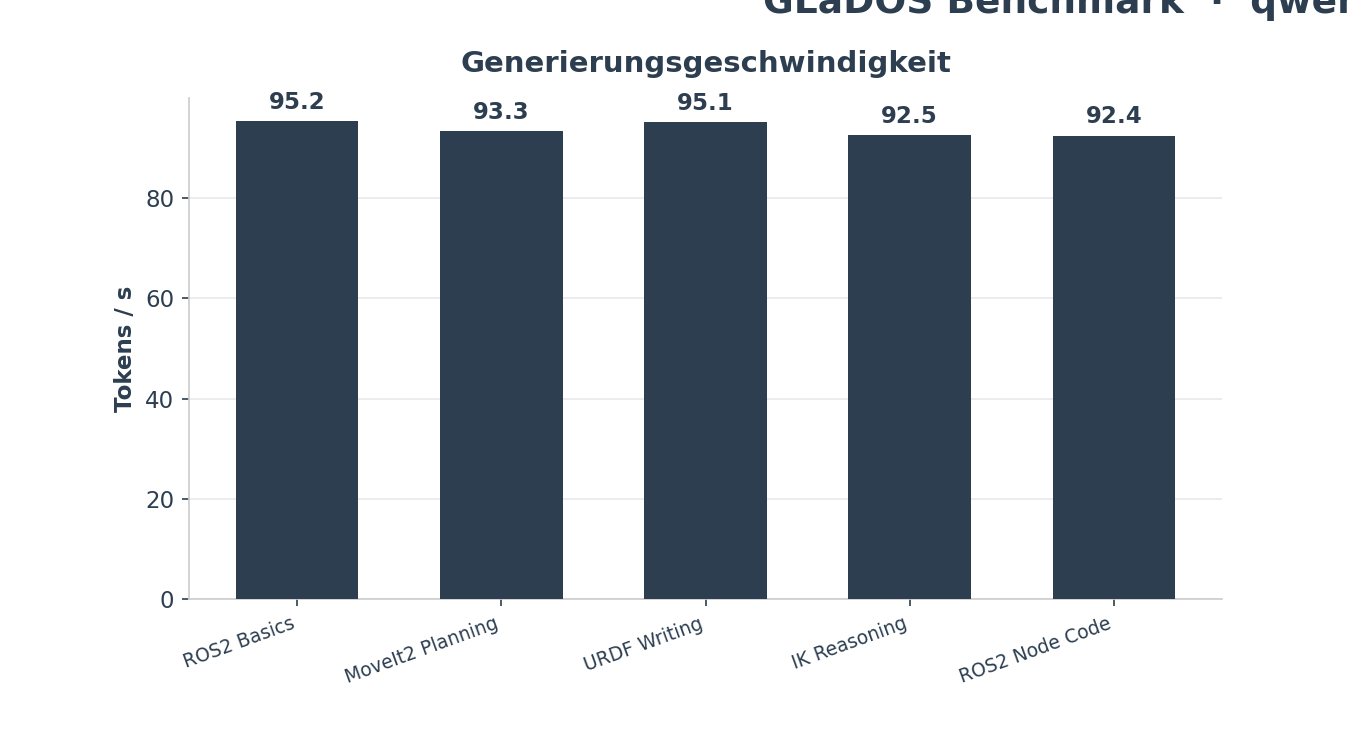
\includegraphics[width=0.85\textwidth]{llm_generierungsgeschwindigkeit.png}
    \caption{Token-Generierungsgeschwindigkeit (Tokens/s) für fünf robotikspezifische Prompts.
    Alle Prompts werden mit einer konsistenten Geschwindigkeit von ca.\,93 Tokens/s verarbeitet.}
    \label{fig:eval_gen_speed}
\end{figure}

Die Generierungsgeschwindigkeit liegt konsistent bei durchschnittlich
\textbf{93,7 Tokens/s} über alle fünf Prompts (Abbildung~\ref{fig:eval_gen_speed}).
Die geringe Varianz ($\pm$\,1,5 Tokens/s) zeigt, dass die Inferenzgeschwindigkeit
weitgehend unabhängig von der Prompt-Komplexität ist, sie hängt
primär von der Speicherbandbreite der GPU ab.

\subsection{Antwortzeit-Aufschlüsselung}

\begin{figure}[H]
    \centering
    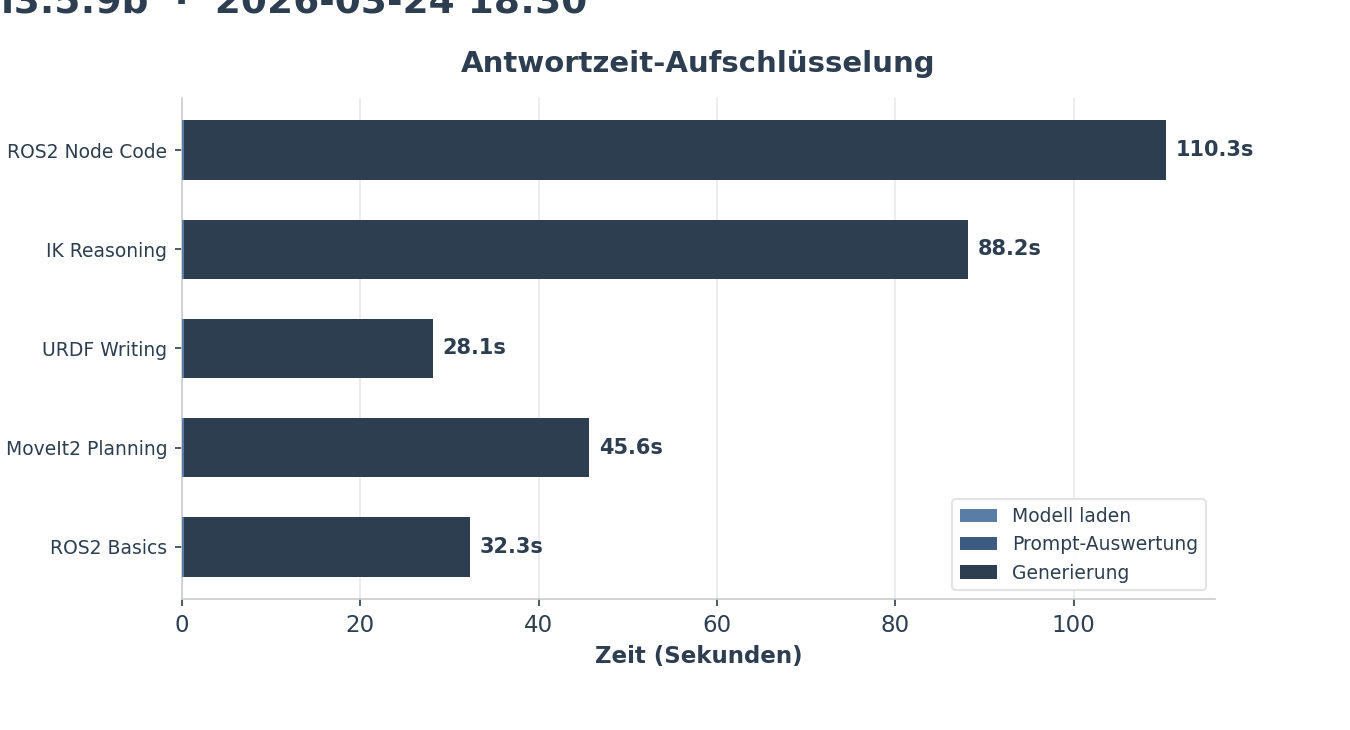
\includegraphics[width=0.85\textwidth]{llm_antwortzeit.png}
    \caption{Zeitliche Aufschlüsselung der Antwortzeiten: Modell laden, Prompt-Auswertung (Prefill) und Generierung. Die Gesamtzeit skaliert linear mit der Antwortlänge.}
    \label{fig:eval_latency}
\end{figure}

Abbildung~\ref{fig:eval_latency} schlüsselt die Antwortzeit auf.
Die Prefill-Phase (Prompt-Auswertung) benötigt nur wenige Sekunden,
während die Generierungsphase proportional zur Antwortlänge skaliert.
Für den längsten Prompt (ROS2 Node Code, $\approx$10.000 Tokens)
beträgt die Gesamtantwortzeit ca.\,110 Sekunden.

\subsection{GPU-Auslastung und VRAM}

\begin{figure}[H]
    \centering
    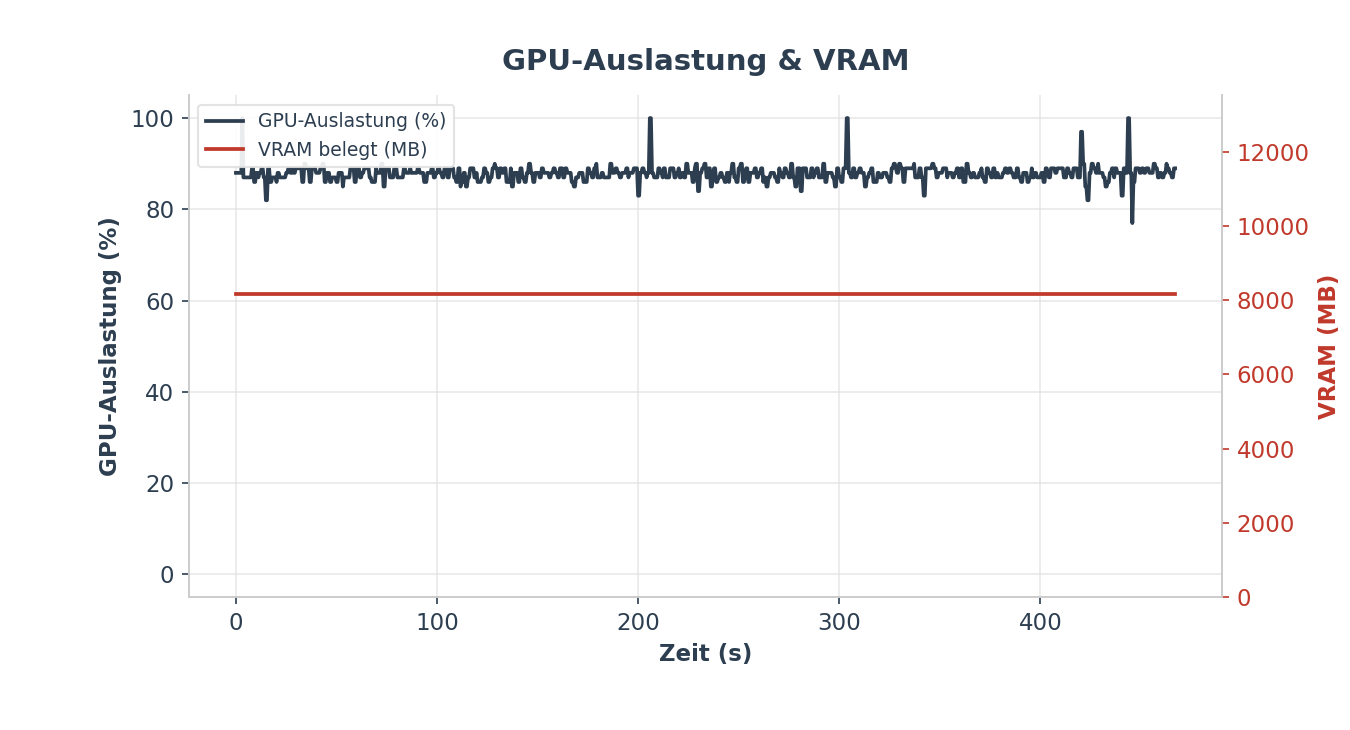
\includegraphics[width=0.85\textwidth]{llm_gpu_vram.png}
    \caption{GPU-Auslastung und VRAM-Belegung während des Benchmarks. Die GPU-Auslastung liegt
    stabil bei ca.\,90\,\%, der VRAM-Bedarf beträgt konstant ca.\,8\,GB.}
    \label{fig:eval_gpu_vram}
\end{figure}

Die GPU-Auslastung liegt während der Inferenz stabil bei ca.\,90\,\%
(Abbildung~\ref{fig:eval_gpu_vram}). Der VRAM-Bedarf des Qwen 3.5 9B
beträgt konstant ca.\,8\,GB und liegt damit deutlich unter dem
12-GB-Limit der RTX 3080 Ti. Der verbleibende VRAM steht für den
KV-Cache und ggf. parallele Prozesse zur Verfügung.

\subsection{CPU- und RAM-Auslastung}

\begin{figure}[H]
    \centering
    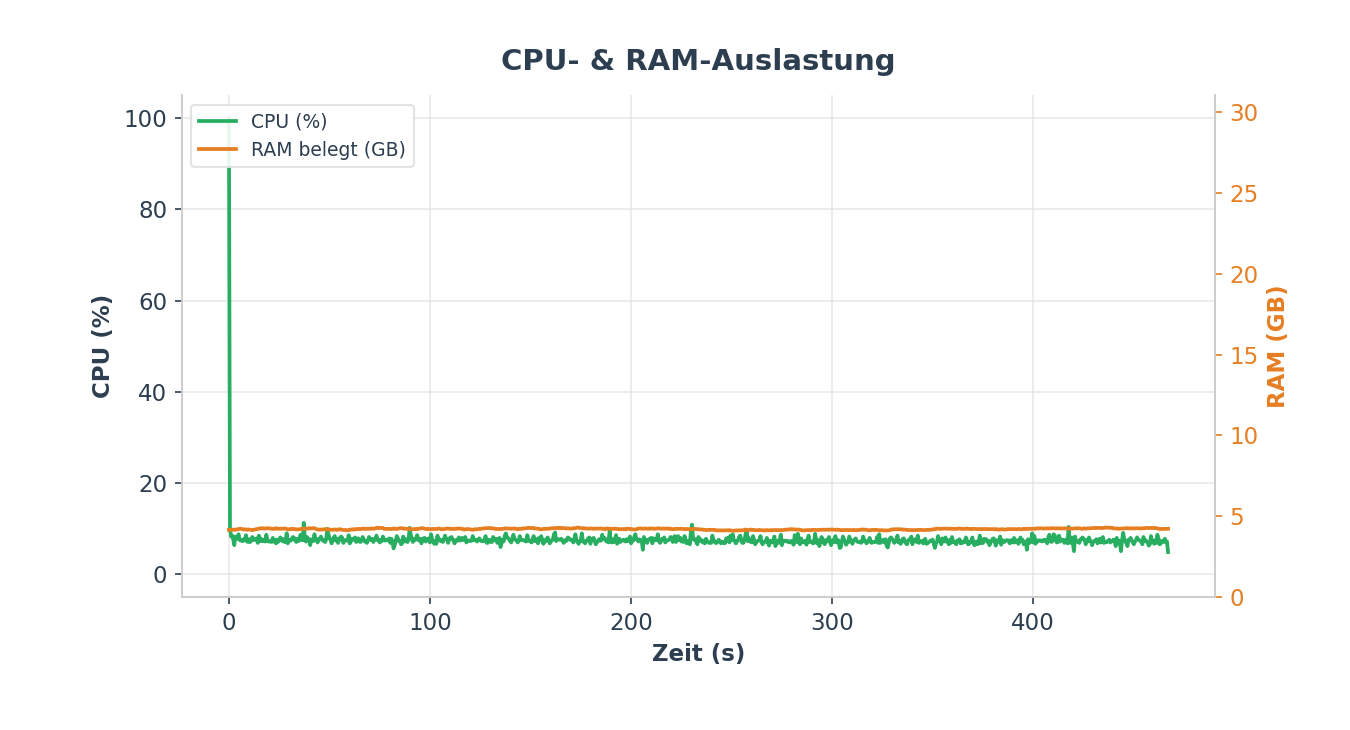
\includegraphics[width=0.85\textwidth]{llm_cpu_ram.png}
    \caption{CPU- und RAM-Auslastung während der LLM-Inferenz. Die CPU-Belastung bleibt
    unter 15\,\%, der RAM-Bedarf bei ca.\,4\,GB.}
    \label{fig:eval_cpu_ram}
\end{figure}

Da die gesamte Inferenz auf der GPU stattfindet, bleibt die CPU-Auslastung
gering ($<$\,15\,\%, Abbildung~\ref{fig:eval_cpu_ram}). Der Arbeitsspeicherverbrauch
ist mit ca.\,4\,GB ebenfalls moderat, was den parallelen Betrieb weiterer
Anwendungen (z.\,B. ROS2-Nodes) ermöglicht.

\subsection{GPU-Leistungsaufnahme}

\begin{figure}[H]
    \centering
    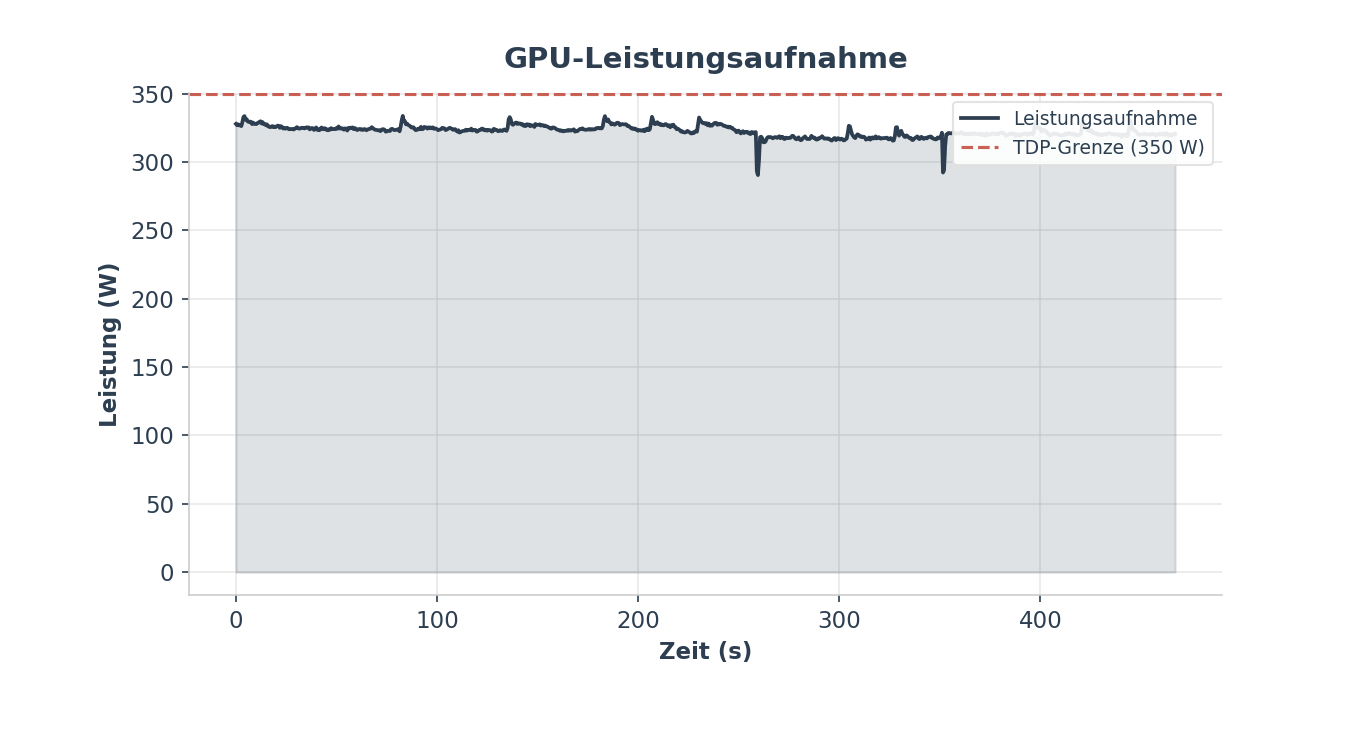
\includegraphics[width=0.85\textwidth]{llm_gpu_leistung.png}
    \caption{GPU-Leistungsaufnahme während des Benchmarks. Die Leistung liegt bei ca.\,320\,W
    (TDP-Grenze: 350\,W), was einer nahezu vollständigen Auslastung der GPU entspricht.}
    \label{fig:eval_gpu_power}
\end{figure}

Die GPU-Leistungsaufnahme beträgt während der Inferenz ca.\,320\,W
(Abbildung~\ref{fig:eval_gpu_power}), was nahe an der TDP-Grenze von
350\,W liegt. Für den Dauerbetrieb ist daher eine ausreichende Kühlung
sicherzustellen.

\subsection{Netzwerk- und Festplatten-E/A}

\begin{figure}[H]
    \centering
    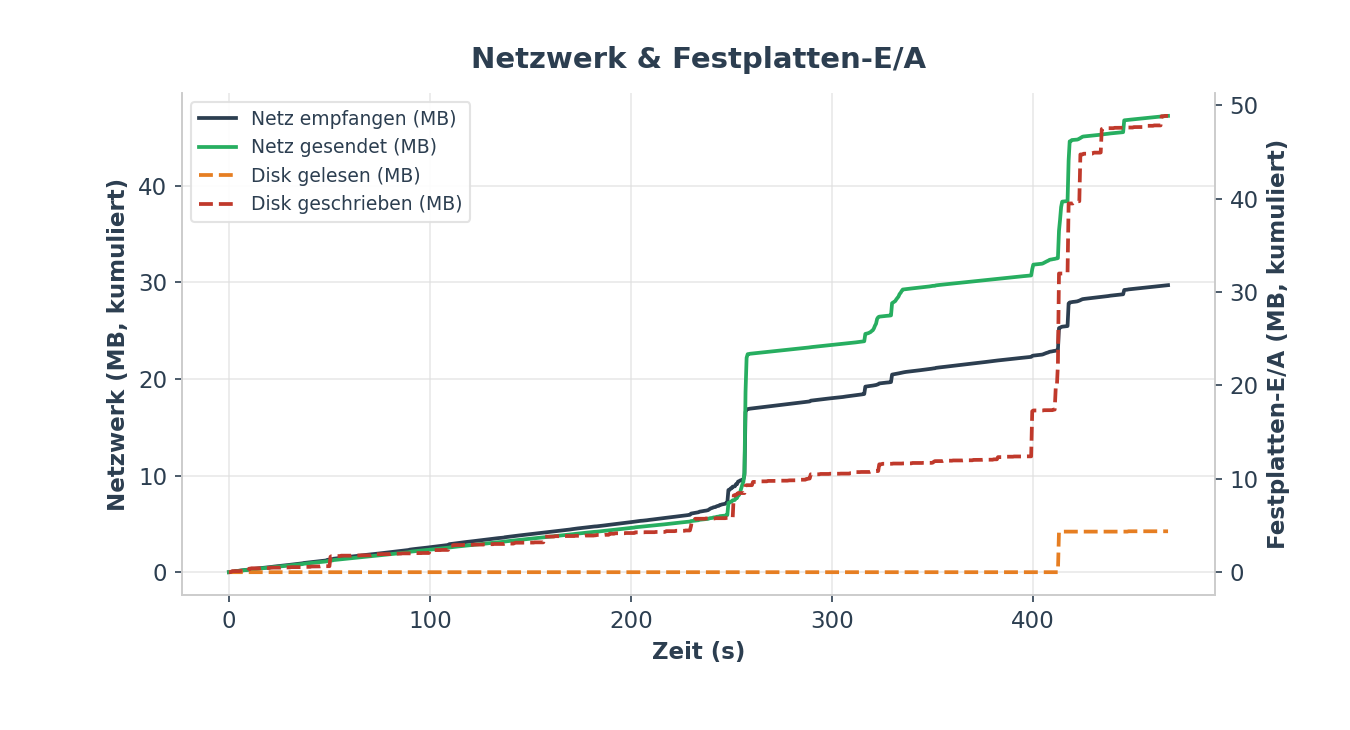
\includegraphics[width=0.85\textwidth]{llm_netzwerk_io.png}
    \caption{Kumulativer Netzwerk- und Festplatten-E/A während des Benchmarks.
    Der Netzwerkverkehr resultiert aus der Kommunikation mit der Ollama-API.}
    \label{fig:eval_io}
\end{figure}

Abbildung~\ref{fig:eval_io} zeigt den kumulativen E/A-Verlauf.
Da das Modell nach dem initialen Laden vollständig im GPU-Speicher
liegt, ist die Festplattenaktivität vernachlässigbar. Der Netzwerkverkehr
resultiert aus der lokalen HTTP-Kommunikation mit der Ollama-API.

% ============================================================
\section{ASR-Benchmark: Parakeet TDT 0.6B}
\label{sec:eval_asr}
% ============================================================

Zur Evaluierung der Spracherkennung wurde eine Testaufnahme mit 14 Sätzen
aus dem robotikspezifischen Kontext (ROS2, igus ReBeL) verwendet.
Die Aufnahme (55\,s, 16\,kHz Mono) wurde durch das Parakeet TDT 0.6B
Modell transkribiert und die Ergebnisse satzweise gegen die Referenztranskription
ausgewertet. Als Metriken dienen die \textbf{Wortfehlerrate} (WER),
die \textbf{Zeichenfehlerrate} (CER) sowie der \textbf{Echtzeit-Faktor} (RTF).

\subsection{Wortfehlerrate pro Satz}

\begin{figure}[H]
    \centering
    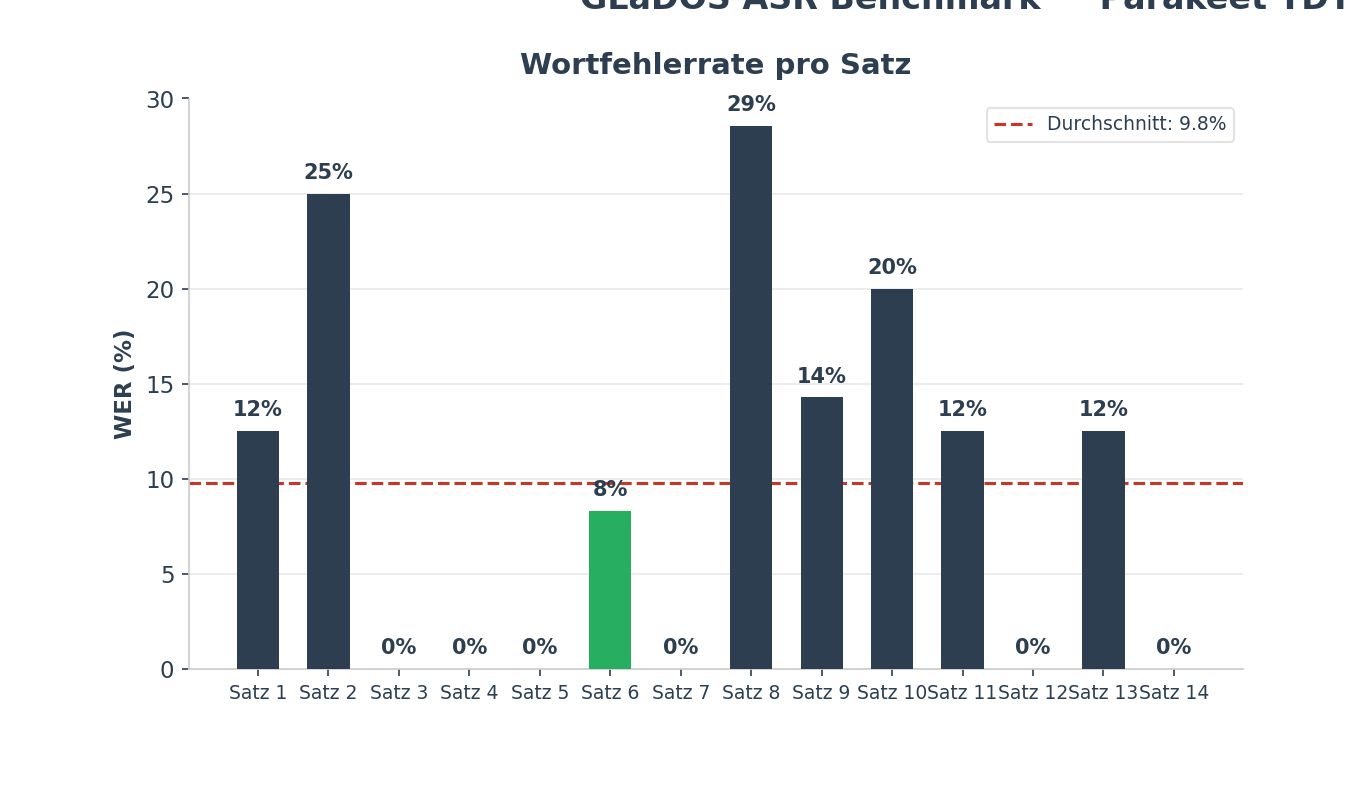
\includegraphics[width=0.85\textwidth]{asr_wer_pro_satz.png}
    \caption{Wortfehlerrate (WER) pro Satz. 6 von 14 Sätzen werden fehlerfrei transkribiert.
    Die durchschnittliche WER beträgt 9,8\,\%.}
    \label{fig:eval_wer}
\end{figure}

Abbildung~\ref{fig:eval_wer} zeigt die WER pro Satz. Die durchschnittliche
Gesamt-WER beträgt \textbf{9,8\,\%}; 6 von 14 Sätzen werden fehlerfrei
transkribiert (WER\,=\,0\,\%). Die höchste Fehlerrate tritt bei Satz~8 auf
(\glqq{}Set the maximum velocity to fifty percent\grqq{}, WER\,=\,29\,\%),
da das Modell die ausgeschriebene Zahl \glqq{}fifty percent\grqq{} als
\glqq{}50\,\%\grqq{} transkribiert.

\subsection{Fehlerverteilung}

\begin{figure}[H]
    \centering
    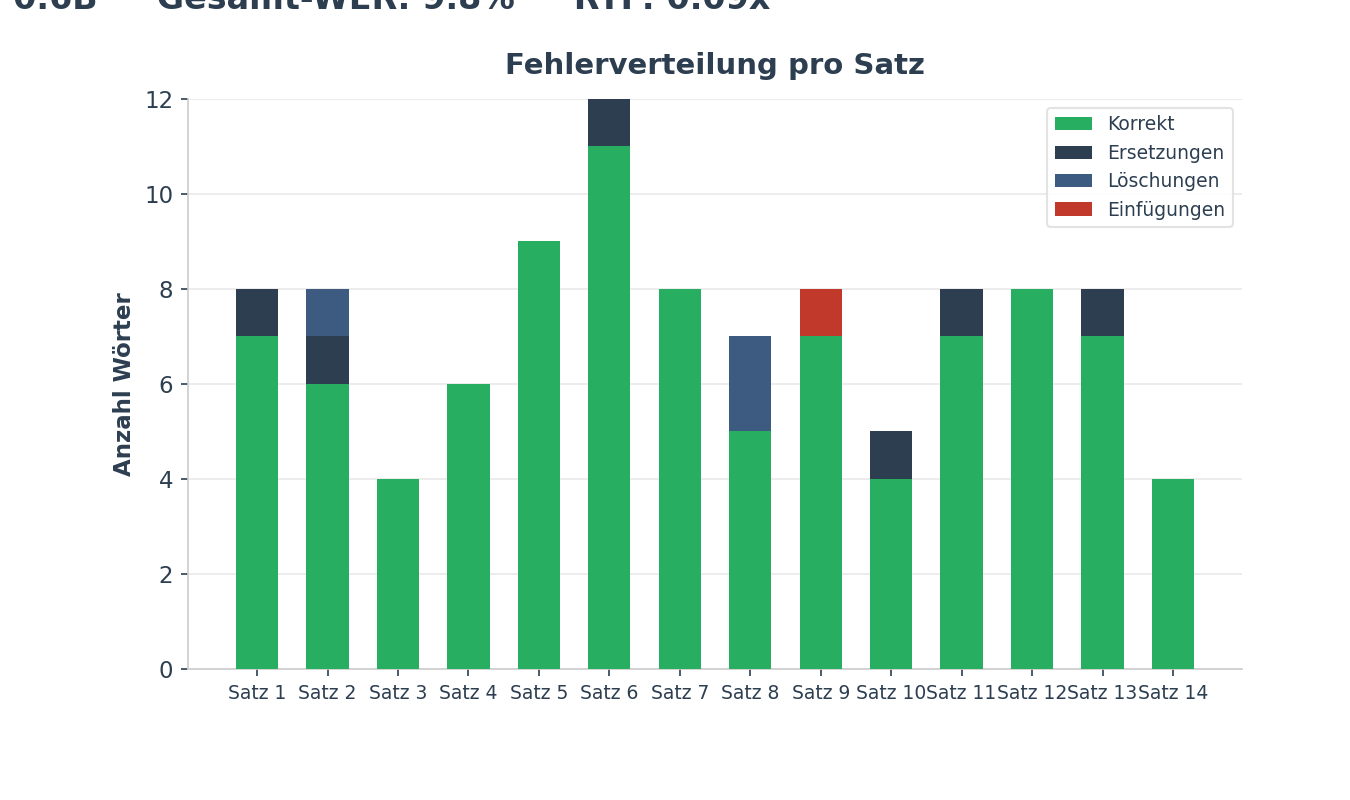
\includegraphics[width=0.85\textwidth]{asr_fehlerverteilung.png}
    \caption{Fehlerverteilung pro Satz: Anzahl korrekter Wörter, Ersetzungen, Löschungen und Einfügungen.
    Die Mehrzahl der Wörter wird korrekt erkannt.}
    \label{fig:eval_error_dist}
\end{figure}

Die Fehleranalyse in Abbildung~\ref{fig:eval_error_dist} zeigt, dass die
dominierenden Fehlerquellen Ersetzungen sind, insbesondere bei domänentypisch fachspezifischen
Eigennamen wie \glqq{}Igus ReBeL\grqq{} (transkribiert als \glqq{}EGOS
Rebel\grqq{}) und \glqq{}MoveIt\grqq{} (transkribiert als \glqq{}MoveId\grqq{}).
Solche Fehler könnten durch ein domänenspezifisches Sprachmodell (Language Model)
oder eine Nachverarbeitungspipeline reduziert werden.

\subsection{WER vs. CER}

\begin{figure}[H]
    \centering
    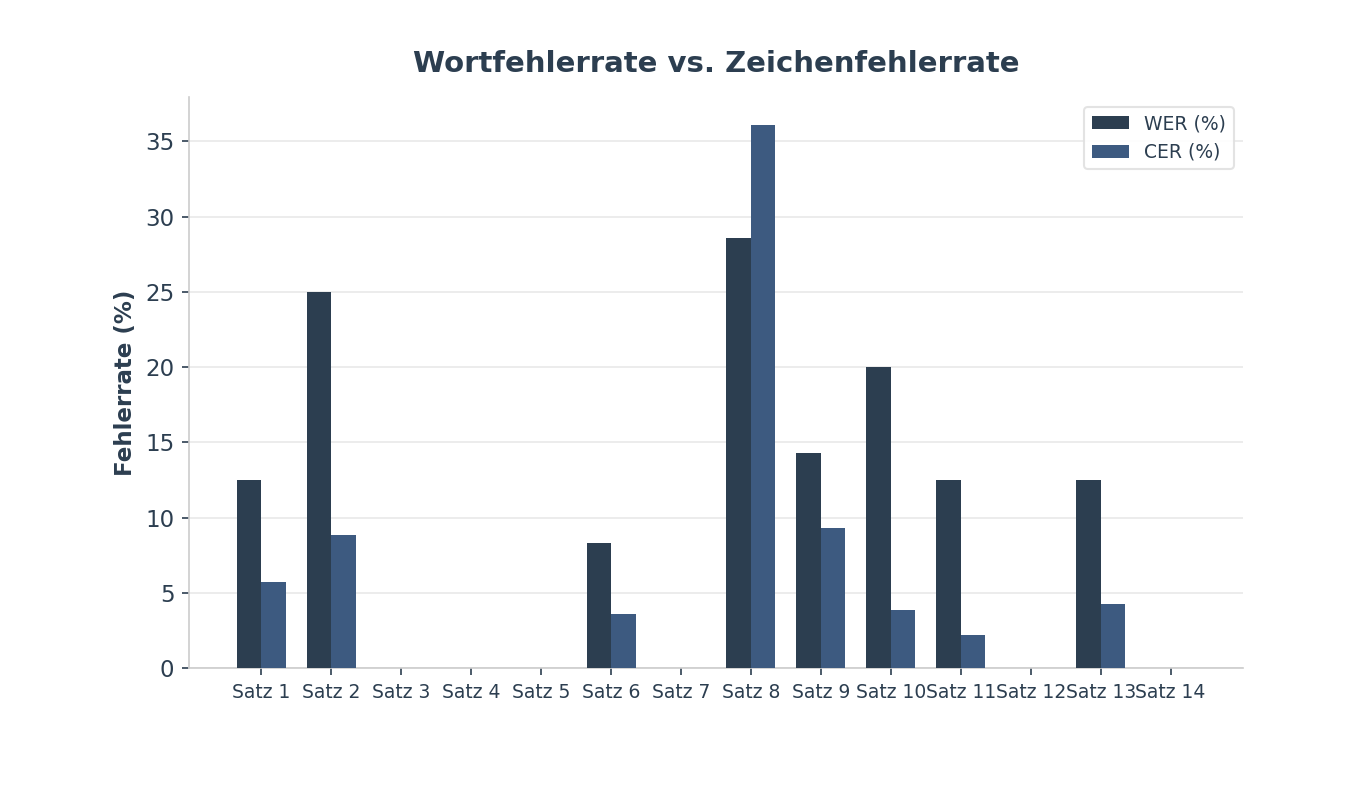
\includegraphics[width=0.85\textwidth]{asr_wer_vs_cer.png}
    \caption{Vergleich von Wortfehlerrate (WER) und Zeichenfehlerrate (CER) pro Satz.
    Die CER liegt durchgehend unter der WER, was auf phonetisch korrekte Transkriptionen hindeutet.}
    \label{fig:eval_wer_cer}
\end{figure}

Abbildung~\ref{fig:eval_wer_cer} vergleicht WER und CER. Die CER liegt
mit \textbf{5,4\,\%} deutlich unter der WER (9,8\,\%), was darauf hindeutet,
dass die meisten Fehler nur einzelne Zeichen innerhalb eines Wortes betreffen
(z.\,B. \glqq{}ReBeL\grqq{} $\rightarrow$ \glqq{}Rebel\grqq{}).
Die phonetische Grundstruktur der Wörter wird weitgehend korrekt erfasst.

\subsection{Zusammenfassung der ASR-Ergebnisse}

\begin{figure}[H]
    \centering
    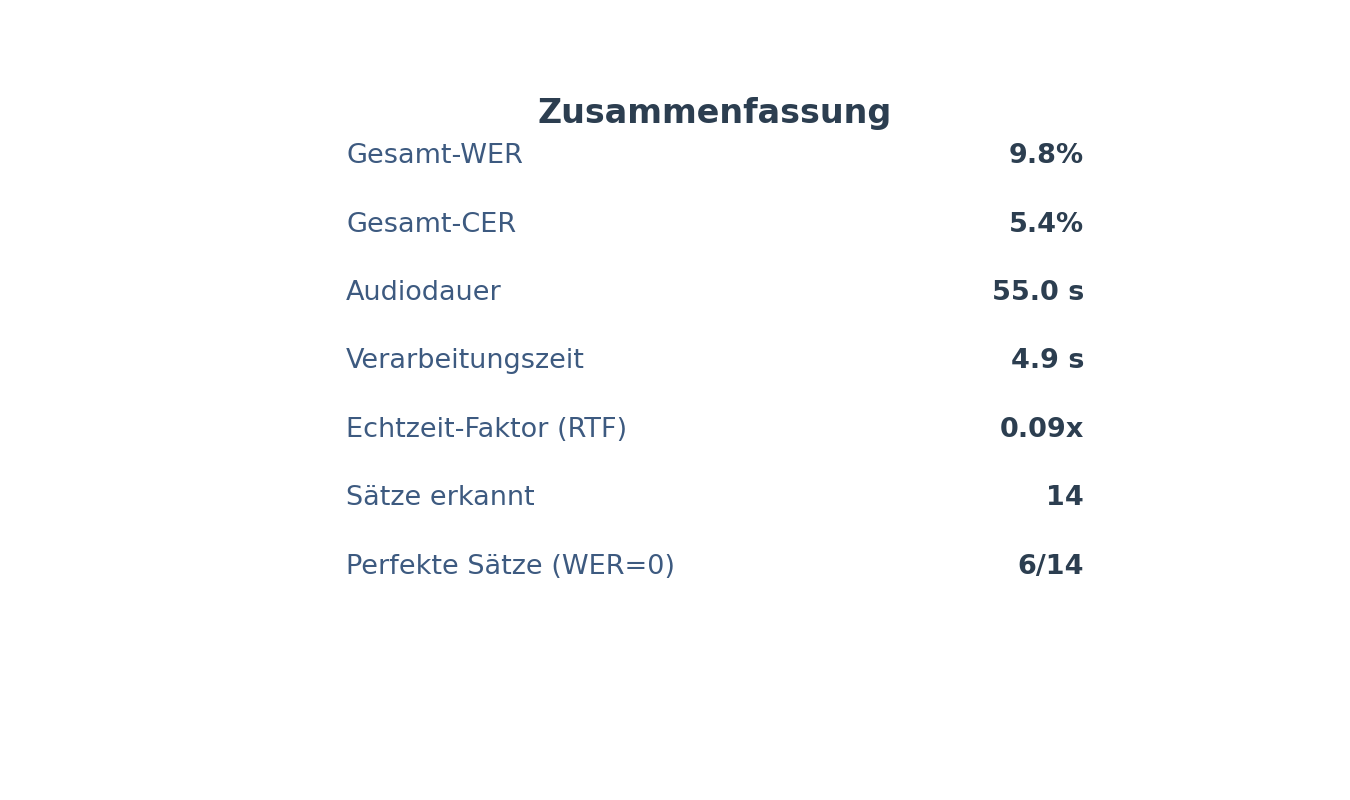
\includegraphics[width=0.85\textwidth]{asr_zusammenfassung.png}
    \caption{Zusammenfassung der ASR-Benchmark-Kennzahlen: Gesamt-WER 9,8\,\%, Gesamt-CER 5,4\,\%,
    Echtzeit-Faktor 0,09x (ca.\,11-fache Echtzeitverarbeitung).}
    \label{fig:eval_asr_summary}
\end{figure}

Die Zusammenfassung in Abbildung~\ref{fig:eval_asr_summary} zeigt die
wichtigsten Kennzahlen. Der Echtzeit-Faktor von \textbf{0,09x} bedeutet,
dass 55 Sekunden Audio in nur 4,9 Sekunden verarbeitet werden, was einer
ca.\,11-fachen Echtzeitverarbeitung auf der CPU entspricht.

% ============================================================
\section{Zusammenfassung der Evaluation}
% ============================================================

\begin{table}[H]
    \centering
    \small
    \begin{tabular}{l l r}
        \toprule
        Metrik & Komponente & Ergebnis \\
        \midrule
        Generierungsgeschwindigkeit & LLM (Qwen 3.5 9B) & 93,7 Tokens/s \\
        VRAM-Belegung & LLM & $\approx$\,8\,GB \\
        GPU-Leistungsaufnahme & LLM & $\approx$\,320\,W \\
        \midrule
        Gesamt-WER & ASR (Parakeet TDT) & 9,8\,\% \\
        Gesamt-CER & ASR & 5,4\,\% \\
        Echtzeit-Faktor (RTF) & ASR & 0,09x \\
        Perfekte Sätze & ASR & 6/14 (43\,\%) \\
        \bottomrule
    \end{tabular}
    \caption{Zusammenfassung der Evaluationsergebnisse.}
    \label{tab:eval_zusammenfassung}
\end{table}

Die Evaluation zeigt, dass die eingesetzte On-Premise-Lösung sowohl bei der
LLM-Inferenz als auch bei der Spracherkennung praxistaugliche Ergebnisse liefert.
Das Qwen 3.5 9B Modell erreicht eine hohe Generierungsgeschwindigkeit von über
90 Tokens/s auf der RTX 3080 Ti, während das Parakeet TDT 0.6B ASR-Modell
eine Gesamt-WER von unter 10\,\% bei 11-facher Echtzeitverarbeitung erzielt.
Die hier gewonnenen Evaluationsergebnisse werden im folgenden Kapitel um
Sicherheits- und Fehlerbetrachtungen ergänzt, die für den produktiven Einsatz
in der Robotik entscheidend sind.

% ============================================================
% Kapitel 7: Ausblick
% ============================================================
\chapter{Fazit und Ausblick}

Zusammenfassend ist zu sagen dass On premise lösungen welche lokal auf server betrieben werden in bestimmmten anwendungsfällen eine sehr gut alternative zu cloud basierten lösungen bieten. Robotikanwendungen in innerbetrieblichen Bereich sind oftmals überschaubar genung bezogen auf veränderlichen variabeln, dass die anpassung der hyperparamter eines klein bis mittlgroßen modells überschaubar sind und demnach gut lokal betrieben werden können. Für große Modelle wie die meißsten sie heute kennen sind große datenzentren nötig mit hohen energiekosten welche für einzelen anwendungen nur wenig sinn ergeben. Dennoch ist immer abzugwwägen ob es in Zukunft für ein wachsendes Unternehmen nicht von Vorteil wäre geld in die hand zu nehmen um eine Serverstruktur zu schaffen welche sich vom Cloud geschäft ein stück weit loslöst und eigen LLM auf eigenen Servern betreibt. Zudem wird trotz wachsender Compute möglichkeiten eine linie nicht überschritten werden können laut \ref{} 


\section{Zusammenfassung der Ergebnisse}
% TODO: Kernerkenntnisse der Arbeit

\section{Ausblick auf die Masterarbeit}
Die Masterarbeit knüpft an vielen der hier erarbeiteten Grundlagen direkt an und umfasst weiterfürhende Themen wie vision language action models in der Robotik. Zusammene mit einer weiteren Forschungs und Entwicklungsarbeit zum Thema ROS2 auf einem IGus Rebel 6 DOf wird ein Testaufbau entwickelt welcher konkret Robotik und Large Languange models im Kontext von Open source und on premise evaluiert.
Generell bleit abzuwarten ob der hype um diese neue Technologie den erhofften wandel der gesellschaft standhalten kann oder doch kompromisse eingegangen werden müssen. auf jden fall wurde durch diese Forschungsarbeit ein Grundstein zur Erklärung der Modelle gelegt.



% ============================================================
% Anhang
% ============================================================
\appendix
% ============================================================
% Anhang
% ============================================================
\chapter{Anhang}

\section{Konfigurationsdateien}
% TODO: Relevante Konfigurationsdateien (z.B. Ollama, GLaDOS)

\section{Testprotokolle}
% TODO: Detaillierte Messprotokolle der Evaluation

\section{Zusätzliche Abbildungen}
% TODO: Ergänzende Screenshots, Diagramme


% ============================================================
% Literaturverzeichnis
% ============================================================
\printbibliography[heading=bibintoc, title={Literaturverzeichnis}]

\end{document}
